\documentclass[letterpaper,12pt]{article}
\usepackage{dgjournal}   % copied from the journal
\usepackage{mathptmx}	% copied from the journal
\usepackage[authoryear,comma,sectionbib]{natbib} % copied from the journal


% packages used in this article
\usepackage{url}
\usepackage{caption}
\captionsetup[figure]{labelfont=bf}
\captionsetup[table]{labelfont=bf}
\usepackage{graphicx}
\usepackage{amsmath, bm}
\usepackage{multirow}

\usepackage{subcaption}


\DeclareMathOperator{\median}{median}
\newcommand{\howmanySamples}{211~}
\newcommand{\howmanylab}{24~}
\newcommand{\howmanyseedlingsample}{60~}
\newcommand{\howmanyleafsample}{60~}
\newcommand{\howmanytissuesample}{91~}
\newcommand{\howmanyseedlingexperiment}{9~}
\newcommand{\howmanyleafexperiment}{5~}
\newcommand{\howmanytissueexperiment}{10~}
\newcommand{\overlapGene}{104~}
\newcommand{\overlapGeneCze}{9~}
\newcommand{\overlapProb}{$4.8\times 10^{-9}$~}
\newcommand{\rankInSeedling}{159~}
\newcommand{\rankInLeaf}{112~}
\newcommand{\rankInTissue}{513~}
\newcommand{\rankTopPctSeedling}{0.7\%}
\newcommand{\rankTopPctLeaf}{0.5\%}
\newcommand{\rankTopPctTissue}{2.2\%}
\newcommand{\SelectFiveGene}{AT1G63110, AT1G79280, AT3G27530, AT4G02560, AT5G53540}
\newcommand{\recalltophundred}{29~}
\newcommand{\recalltopthousand}{98~}
\newcommand{\recallrankcorrelation}{0.97~}
\title{Identifying stably expressed genes from multiple RNA-Seq data sets}
\date{} % Today's date or a custom date




\begin{document}
	
	
	\author{
		LastName1, FirstName1\\
		\texttt{first1.last1@xxxxx.com}
		\and
		LastName2, FirstName2\\
		\texttt{first2.last2@xxxxx.com}
	}

%Our main points include: 
%\begin{enumerate}
%    \item using multiple (a larger number of) public-available existing/past data sets, 
%	\begin{enumerate}
%	    \item
%		using multiple data sets 
%		\begin{enumerate}
%		    \item
%			as compared to using a single data set: a numerical
%			measure of expression stability (typically, measures
%			of certain aspects of RNA-Seq count variation) can be
%			more reliably estimated by using more data sets (???)
%		    \item
%			(leaf) learn variance components (see GLMM)
%		    \item
%			(leaf) using top 1000 identified genes for
%			normalization.
%		    \item
%			(discussion) use as prior information in Bayesian analysis or
%			use the  set for quality control/vanity check purpose
%		\end{enumerate}
%	    \item
%		(caveat) genes that are stable under a range of conditions
%		might not be the most stable under a particular condition
%		(under a single experiment).
%		\begin{enumerate}
%		    \item
%			(leaf) identify different reference sets for different tissue
%			types
%		\end{enumerate}
%
%	    \item Subtle points on interpretability and comparability (??? do
%		we need some toy examples)
%
%		\begin{enumerate}
%		    \item
%			using an explicit reference set: improve interpretability
%		    \item
%			using a common reference set (when comparing two or more studies): improve comparability
%		\end{enumerate}
%	\end{enumerate}
%
%    \item
%	using a numerical measure of stability
%	\begin{enumerate}
%	    \item
%		(leaf) stability of house-keeping genes (HKGs)
%	    \item
%		(leaf) different numerical measures (geNorm, normFinder)
%	    \item
%		(leaf) different data sources (microarray and RNA-Seq)
%	    \item
%		(discussion) numerical measure of stability vs biological
%		stability 
%	\end{enumerate}
%
%
%    \item
%	Validate the stably expressed genes that we find? (no leaf yet) 
%	\begin{enumerate}
%	    \item
%		biological function (online database) 
%	    \item
%		(GO analysis)
%	\end{enumerate}
%
%    \item
%	Future, use our methods and leaf (stable set, rankings, variance
%	components) in real studies.
%\end{enumerate}

\newpage
% \maketitle

\begin{center}
% {\Large Identification of stably expressed genes from Arabidopsis RNA-Seq data}\\

{\Large Identifying stably expressed genes from multiple RNA-Seq data sets}

\today

\end{center}


\newpage
\section*{Abstract}
We examined RNA-Seq data on \howmanySamples biological samples from \howmanylab different
experiments carried out by different labs and identified genes that are stably
expressed across biological samples, treatment conditions, and experiments. We
fit a Poisson log-linear mixed-effect model to the read counts for each gene
and decomposed the total variance into between-sample, between-treatment and
between-experiment variance components. Identifying stably expressed genes is
useful for count normalization and differential expression analysis. The
variance component analysis that we explore here is a first step towards understanding the sources
and nature of the RNA-Seq count variation.
When using a numerical measure to identify stably expressed genes, the outcome
depends on multiple factors: the reference sample sets used, the technology
used for measuring gene expression, and the specific numerical stability
measure used.  Since DE is measured by relative frequencies, we argue that DE
is a relative concept. We advocate using an explicit reference gene set for
count normalization to improve interpretability of DE results, and recommend
using a common reference gene set when analyzing multiple RNA-Seq experiments
to avoid potential inconsistent conclusions.


% cited from the abstract of the paper: " Real-time PCR (qPCR) is the most
% accurate method of quantifying gene expression, provided that suitable
% endogenous controls are used to normalize the data"

\section{Introduction}\label{section:Introduction}

RNA sequencing (RNA-Seq) has become the technology of choice for transcriptome
profiling over the last few years. The exponential growth in RNA-Seq studies have
produced a large amount of \textit{Arabidopsis thaliana} (Arabidopsis) data under a variety of experimental/environmental conditions.  It is only natural to begin exploring
how the large amount of existing data sets can help the analysis of future
data.  In this paper, we discuss identifying stably expressed genes from
multiple existing RNA-Seq data sets based on a numerical measure of stability.
We envision that such identified stably expressed genes could be used as a
reference set or prior information for count normalization and differential
expression (DE) analysis of future RNA-Seq data sets obtained from similar or
comparable experiments.  We also fit a random-effect model to the read counts
for each gene and decompose the total variance to into between-sample,
between-treatment and between-experiment variance components. The variance component
analysis is a first step towards understanding the sources and nature of the
RNA-Seq count variation.  To illustrate our methods, we examined RNA-Seq data
on \howmanySamples Arabidopsis  samples from \howmanylab different experiments carried out by
different labs and identified genes that were stably expressed across
biological samples, experimental or environmental conditions, and experiments
(labs).  

A reference set of stably-expressed genes will be useful for count
normalization.  A key task of RNA-Seq analysis is to detect DE genes under
various experimental or environmental conditions. Count normalization is
needed to adjust for differences in sequencing depths or library sizes (total
numbers of mapped reads for each biological sample) due to chance variation in
sample preparation.  In DE analysis, gene expression levels are often
estimated from relative read frequencies. For this reason, normalization is also 
needed to account for the fact that non-differentially expressing genes may exhibit
 an apparent reduction or increase in relative read frequencies due to the respective 
 increased or decreased relative read frequencies of truly differentially expressing genes.
 Many existing normalization methods, such as the trimmed
mean of M-values normalization method (TMM) \citep{robinson2010scaling} and
Anders and Huber's normalization \citep{anders2010differential}, assume that the
majority of the genes within an experiment are not DE, and examine the sample
distribution of the fold changes between samples.
% There are two obvious
% difficulties when using such a normalization method: 1) There is great
% uncertainty in observed fold changes.  
% is typical available sample size in any single experiment can be too small
% for us to reliably estimate true fold changes.  
If the experiment condition can affect expression levels of more than half of
the genes, many of the existing normalization methods may be unreliable
\citep{loven2012revisiting, wu2013use}.  This difficulty could be
alleviated if one could identify a set of stably expressed genes whose
expression levels are known or expected to not vary much under different
experimental conditions. Our idea is to identify such a reference set based on
a large number of existing data sets.

Our basic intuition is that a numerical quantification of expression
stability---which typically measures certain aspects of RNA-Seq count
variation---can be more reliably estimated by using more data sets.  There is,
however, a caveat to this idea: as pointed out by \cite{fernandes2008selection} and \cite{hruz2011refgenes},
% stably expressed genes identified under a wide range conditions may show more
% variability under a more specific biological context than those genes
% identified under that particular context.
universally stably expressed genes may not exist. \cite{hruz2011refgenes} showed that a subset of stably
expressed genes from a specific biological context may have more variability
than other genes if examined across a broader range of samples and conditions.
Many studies have shown that stably expressed genes are subject to change from
one experiment to another due to different experimental protocols, different
tissue types, or other varying conditions \citep{reid2006optimized,
hong2010identification}.  The top 100 stably expressed genes in the Arabidopsis
developmental series of \citet{czechowski2005genome} shared only 3 genes with the
top 50 stably expressed genes identified from Arabidopsis seed samples by
\citet{dekkers2012identification}.  In this study, we try to balance
generality and specificity by identifying different reference gene sets for
different tissue types of Arabidopsis. 



We can also consider that when a normalization method is applied to a single data
set, it effectively specifies an implicit reference set of stably expressed
genes (those genes that have the least variation after normalization). From this perspective,
 we can view commonly used normalization techniques as using an internally identified reference 
 set of genes. In contrast, what we are
proposing is that one could alternatively identify a reference set externally by looking
at past data sets. The internally and externally identified reference gene
sets will provide different contexts for the DE analysis: in other words, one
can choose to answer different scientific questions by using different
reference sets. In any case, we advocate  making the reference set explicit
during a DE analysis and using a common reference set when analyzing multiple
datasets. 

% We will further discuss these points in the discussion Section \ref{section:discussion}.


We want to clarify that having stable gene expression is not
equivalent to maintaining a stable biological function.
% a distinction between numerical stability and biological stability---
Often times, we may not
understand the biological functions of genes with numerically stable
expression measures. From an operational point of view, however, numerical
stability is more tractable. In pre-genomic era, the so-called ``\textit{house-keeping
genes}" were often considered to be candidate reference genes for
normalization \citep{bustin2002quantification, andersen2004normalization}. House-keeping
genes are typically constitutive genes that
maintain basic cellular function, and therefore are expected to express at
relatively constant levels in non-pathological situations.  However, many
studies have shown that house-keeping
genes are not necessarily stably expressed according to
numerical measures (a review can be found in \cite{huggett2005real} and
reference therein).  For example, in the microarray analysis of Arabidopsis, \cite{czechowski2005genome}
showed that traditional house-keeping
genes such as ACT2, TUB6, EF-1$\alpha$ are not stably
expressed, and thus not good reference genes for normalization.  Spike-in
genes  have also been considered as reference genes for normalization, but %\citep{jiang2011synthetic}, but
\cite{risso2014nat} showed that spike-in genes are not necessarily stably
expressed according numerical measures either.  
% HKGs or spike-in genes thus cannot be taken as granted as stably expressed
% genes for count normalization purpose.  and careful evaluation should be
% performed when they are being used in normalization. (??? simplify, make
% concise)
%\textbf{Numerically finding stably expressed genes.}
% Why would we bother to study them under RNA-Seq since there are related
% works in microarray} (some sentense are needed to connect the two
% paragraphs)

In this paper, we identify stably expressed genes from RNA-Seq data sets based
on a numerical measure---the sum of three variance components estimated from a
mixed-effect model. 
For microarray data, there have been many efforts to numerically find stably
expressed genes by quantifying the variation of measured expression levels
across a large number of microarray data sets.  For example,
\cite{andersen2004normalization} used a linear mixed model to estimate the
between-group and within-group variances from expression profiles of
microarray experiments, and then quantified expression stability by combining
the two variance components using a Bayesian formulation. 
% For a future experiment, the stability value for a given gene is
% defined as the absolute value of posterior mean plus one standard prediction
% deviation of that gene.  
\cite{czechowski2005genome} measured the expression stability of each gene
using the coefficient of variation (CV). Genes with lower CVs are considered
 more stably expressed.  By investigating 721 arrays under 323 conditions
throughout development, \cite{czechowski2005genome} suggested stably expressed
(reference) genes under different experimental conditions for Arabidopsis.
% find stably expressed genes based on 526. 
%and  validated a subset of most stably expressed genes they identified.
%Similar studies were carried out for Arabidopsis seed
\cite{stamova2009identification},  \citet{dekkers2012identification}, \citet{gur2009identification}, and
 \citet{frericks2008toolbox} screened a large number of microarray data sets
 to identify stably expressed genes in human blood, Arabidopsis seed, breast tumor tissues,
 and mice respectively.
% Similar studies were carried out for Arabidopsis seed
% \citep{dekkers2012identification}, breast tumor
% tissues\citep{gur2009identification}, mouse (universal)
% \citep{frericks2008toolbox} and so on.  
Validation experiments \citep{czechowski2005genome,
dekkers2012identification, huggett2005real,stamova2009identification} showed
that these genes are more stably expressed than traditional house-keeping
genes.  

%The rest of the paper is organized as follows: in Section
%\ref{section:Methods}, we describe the data preparation steps and our method
%of identifying stably expressed genes; in Section \ref{section:Results}, we
%discuss the stably expressed genes and factors that might affact stability
%ranking; we also discuss results from variance component analysis and how to
%use the identified stably expressed genes for count normalization. (AND
%DISCUSSION...)

Our vision is that identifying stably expressed genes is the first step
towards integrative analysis of multiple RNA-Seq experiments. It will help to
answer fundamental questions related to  comparability, reproducibility and
replicability of RNA-Seq experiments.

\section{Methods} 
\label{section:Methods}
In Section \ref{section:DataCollection}, we describe the steps for collecting
and processing RNA-Seq data sets from Arabidopsis experiments.  In Section
\ref{section:countNormalization}, we discuss count normalization methods and
how to apply them to a subset of stably expressed genes.
In Section \ref{subsection:OurMethod},  we introduce the generalized linear
mixed model (GLMM, \citealt{mcculloch2001generalized}) for estimating three
variance components from RNA-Seq data: the \textit{between-sample},
\textit{between-treatment} and \textit{between-experiment} variances.  We
define the \textit{total variance} measure for expression stability as the sum
of estimated variance components.  In Section
\ref{subsection:OtherStabilityMeasure}, we review the CV and M-value measures
for gene expression stability.



\subsection{RNA-Seq data collection and processing}\label{section:DataCollection} 

\subsubsection*{Overview of the RNA-Seq data sets}
We examined RNA-Seq data from 49 Arabidopsis experiments stored on the NCBI
GEO repository (see more details below). After screening, we retained data
from \howmanySamples biological samples in \howmanylab experiments.  To illustrate our methods
for finding stably expressed genes, we divided the experiments into three
groups: \textit{the seedling group} contains \howmanyseedlingsample Arabidopsis seedling samples
from \howmanyseedlingexperiment experiments; \textit{ the leaf group} contains \howmanyleafsample Arabidopsis leaf
samples from \howmanyleafexperiment experiments;  the \textit{multi-tissue group} contains \howmanytissuesample
samples from \howmanytissueexperiment experiments on multiple tissue types (shoot apical, root tip,
primary root, inflorescences and siliques, hypocotyl, flower, carpels, aerial
tissue, epidermis, seed).  Table \ref{table:TableSet3} summarizes the basic information about
the three groups.
% lowly-expressed genes provide little information about expression level, and 
\begin{table}[!ht]
    \centering
    \caption{Summary statistics for the three groups of Arabidopsis samples.}
    \begin{tabular}{lp{2.4cm}p{2.3cm}p{2cm}p{1.5cm}} \hline
	Group & \#  experiments & \# treatments  & \# samples & \# genes \\ \hline
	seedling &   9 &  27 &  60 & 22207 \\ 
	leaf &   5 &  28 &  60 & 20967 \\ 
	multi-tissue &  10 &  39 &  91 & 23611 \\ \hline
	\label{table:TableSet3}
    \end{tabular}
\end{table}

To find stably expressed genes in each group, we processed the raw
sequencing data and summarized the results as count matrices of mapped RNA-Seq
short reads (see details below).  We removed genes with low mean numbers (less
than 3) of mapped read counts for all experiments.  Such genes tend to be more prone to sequencing
noise, less interesting to biologists, and also cause convergence issues when
fitting statistical models. Many other researchers (such as \citealt{anders2013count})
recommend removing such genes before analyzing RNA-Seq data.  The number of
remaining genes in each group is also summarized in Table
\ref{table:TableSet3}.


\subsubsection*{Details of the data processing steps}
The \textit{Gene Expression Omnibus} (GEO) repository at \textit{National
Center for Biotechnology Information} (NCBI,
\url{http://www.ncbi.nlm.nih.gov/}) stores raw sequencing data from a large
number of RNA-Seq experiments.  For this study, we restrict our attention to
Arabidopsis experiments satisfying the following conditions: 1.  Ecotype =
``Columbia" (we kept only the Columbia samples from experiments that compare
Columbia samples to other ecotypes); 2. There are at least two treatments and 2 biological replicates for each
treatment; 3. Library strategy= ``RNA-Seq"; 4.
Library source = ``transcriptomic"; 5.  Library selection= ``cDNA"; 6.  Library
layout = ``Single end"; 7. If there are repeated measurements over time, we choose samples from one time point. 

 We screened all the Arabidopsis experiments available from the NCBI
GEO repository up to May 31, 2015 and downloaded raw RNA-Seq data (Sequence Read Archive files)
from 49 experiments. % Each data set is named by its unique accession number. 

 
We assembled our own in-house pipeline to process all the raw RNA-Seq data:
align the raw RNA-Seq reads to the reference genome and summarize the read counts at the 
gene level. In the GEO repository, the
mapped read counts are unavailable for some experiments and the available ones
are from different processing pipelines.  
Our pipeline, implemented using the software R \citep{Rpackage}, is summarized as follows: 
\begin{enumerate}
    \item Convert the Sequence Read Archive (SRA) files to FASTQ files using the NCBI SRA Toolkit (\cite{leinonen2010sequence}, version 2.3.5-2).
     %\url{http://www.ncbi.nlm.nih.gov/Traces/sra/sra.cgi?cmd=show&f=software&m=software&s=software}). 
    \item Download the reference genome 
         \begin{quote}
    	\verb|Arabidopsis_thaliana.TAIR10.22.dna.toplevel.fa |
    \end{quote} 
    from the \textit{ Ensembl plants FTP server} (\url{http://plants.ensembl.org/info/data/ftp/index. html}) and build index using \verb|build()| function from 
    Subread aligner (RSubread, version 1.16.2, \citealt{liao2013subread}) in the software R
    \citep{ Rpackage}. The index allows fast retrieval of the sets of positions in the reference genome where the short reads are more likely to align. 
    \item Align short reads in FASTQ files to the Arabidopsis reference genome using the \verb|align()| function from Rsubread. 
 %As suggested by\cite{anders2013count}, "FASTA(DNA)" link was chosen because
 %samples were aligned to the genome. .  
 \item
     Summarize the read counts at the gene level using the \verb|featureCounts()| function from the
     Subread aligner
     % using annotation \verb"Arabidopsis_thaliana.TAIR10.22.gtf" 
     and store the read counts as data matrix.  
     % Default options for all functions were used The
     The annotation file 
     \begin{quote}
     \verb"Arabidopsis_thaliana.TAIR10.22.gtf" 
 \end{quote}
     is downloaded from Ensembl plants FTP server. The multi-mapping or
     multi-overlapping reads were not counted.  

\end{enumerate}
Subread aligner is a recently developed sequence mapping tool that adopts a
seed-and-vote paradigm to map the RNA-Seq short reads to the genome. 
It breaks each short read into a series of overlapping segments called
subreads and uses the subreads to vote on the optimal genome location of the
original read. The subreads are shorter and can be mapped to the genome much
faster.
Compared to other aligners such as Bowite 2 \citep{langmead2012fast} or BWA
\citep{li2009fast}, Subread aligner is both faster and more accurate
\citep{liao2013subread}. We compared results from the above
pipeline to results from a pipeline described in \cite{anders2013count} over several RNA-Seq experiment data, and Rsubread
was more than three times faster and successfully mapped more reads to the
reference genome.  For researchers familiar with R, it also has the advantage
that it is completely implemented in R.

% pipelines are Poisson (???, similar as read counts from two technical
% replicates).


%(\textbf{Three groups of experiments}) \cite{czechowski2005genome}, \cite{hruz2011refgenes}, and
%\cite{dekkers2012identification} show that gene expression vary across
%different tissue types and development stages. For this reason, 
We divided the experiments into three groups as summarized in Table 1.  As an
additional data quality control measure,  we keep an experiment only when it 
has mapping quality (number of successfully mapped reads divided by total number of reads) $\geq 50\%$ for all samples.
Then within each group, we computed an
initial set of normalization factors from all samples combined using the method
described in Section \ref{section:countNormalization}.  An experiment is
retained only when the normalization factors of all samples in the experiment
are between 0.50 and 1.50.  If the initial estimated normalization factor is
too different from 1 for a sample, it often indicates that the read counts
distribution in the corresponding sample is markedly different from the
distributions of the rest of the samples. Such samples demand additional
attention before being incorporated in the studies that we intend to do.


%\textbf{Moved from introduction part, or better to put it in discussion part?}
%\cite{czechowski2005genome} and \cite{dekkers2012identification} adopted similar approach for statistical analysis for identifying stably expressed genes, and both used Arabidopsis microarray data. Briefly, for each gene the mean expression and the standard deviation (SD) over all biological samples are calculated, and the coefficients of variation (CV), which is the ratio of SD to mean expression, are obtained. Genes with lower CVs are expected to be more stably expressed. This simple approach, however, does not provide us any information about possible sources, except the amounts,  of variation.  \textbf{}\\ 

\subsection{Count normalization}\label{section:countNormalization}
As explained in the introduction, count normalization is needed when analyzing RNA-Seq data to
 1) adjust for differences in sequencing depths or
library sizes; 2) to adjust for the apparent changes in relative read
frequencies of non-DE genes that occur as a consequence of changes in relative read frequencies of truly DE genes.

For the second type of adjustment, we follow Anders and Huber's method
\citep{anders2010differential} for 
estimating normalization factors.  Let $y_{ij}$ denote the read count
for $i$th gene of the $j$th sample ($m$ genes and $n$ samples in total). We first
create a pseudo-reference sample where each gene's expression value is the 
geometric mean expression over all real samples for that gene,
\begin{equation}
 y_{i,0} = (\prod_{j=1}^ny_{i,j})^{1/n},  i=1, \ldots, m. 
\end{equation} 
Next we calculate the median fold-change in relative frequency between
each sample $j$ and the pseudo-reference sample,
\begin{equation}\label{eq:normfactors} 
    R'_j = \median \left(\dfrac{y_{1,j}/N_j}{y_{1,0}/N_{0}}, \ldots, \dfrac{y_{m,j}/N_j}{y_{m,0}/N_{0}}\right),
\end{equation}
where $N_j$ is the library size for sample $j$ (the sum of RNA-Seq
counts mapped to all genes retained in each sample). Finally, the
\textit{normalization factor}  $R_j$ for sample $j$ is calculated as 
\begin{equation}
    \label{eq:norm3}
R_j = \dfrac{R'_j}{(\prod_{j=1}^{n}R'_j)^{1/n}}.
\end{equation}
Using the estimated normalization factors, the relative frequencies will be
computed as $y_{ij}/{N_j R_j}$, which we will call the \textit{normalized relative frequency}
 for gene $i$ in sample $j$. The assumption made here is that the
median fold change between normalized relative frequencies in two samples should be 1. In
other words, this normalization method assumes that the majority of genes are
not DE. The NBPSeq package \citep{di2014package} has an inbuilt function for
this procedure and it will be used for count normalization in this paper. With
the estimates from equation~(\ref{eq:norm3}), we see that the median fold
change in normalized relative frequencies between each sample and the pseudo-reference
sample will be set to 1:
\begin{equation}
    \label{eq:medianfc}
    \median \left(\dfrac{y_{1,j}/ N_jR_j}{y_{1,0}/N_{0}R_0}, \ldots,
    \dfrac{y_{m,j}/N_j R_j}{y_{m,0}/N_{0}R_0} \right) = 1,
\end{equation}
where $R_0 = (\prod_{j=1}^{n}R'_j)^{-1/n}$.

%% We will apply Anders and Huber's method to a subset of stably expressed genes
% we identify based on our stability measure. For this purpose, 

We can apply equation~(\ref{eq:normfactors}) to a subset of reference genes to
estimate normalization factors.  In doing so,  effectively, the median fold
change in equation~(\ref{eq:medianfc}) among the reference genes will be set
to 1 in each sample $j$.
% ??? We will call the median fold changes in equation (4) the reference median fold changes. ???  
Other normalization methods may make different assumptions
than Anders and Huber's, but some assumptions of a similar nature seem
unavoidable.  For example, the TMM method of \citet{robinson2010scaling} is
based on a similar principle: assuming the majority of the genes are not DE.
The TMM method can be applied to a subset of genes selected based on an
initial screening of mean expression level and fold changes. In TMM method,
one can also specify certain quantile (instead of the median) of the fold
changes to be 1.

In this paper, we will identify stably expressed genes from multiple data sets
based on numerical measure and use them as reference for estimating
normalization factors (from equations~(\ref{eq:normfactors}) and~(\ref{eq:norm3})). 
However, to identify the stably expressed genes, we first
need a set
of initially estimated normalization factors.  To tackle this circular
dependence, we use a one-step iteration method to estimate the normalization
factors: 
\begin{enumerate}
    \item
	First, we use all the genes to calculate the initial normalization factors; 
    \item
	Then, we fit a GLMM to each gene and estimate the total variance measure, incorporating the initial normalization factors as
	an offset term (see Section \ref{subsection:OurMethod}); 
    \item
	Next, we select the top 1000 stably expressed genes based on the total
	variance measure estimated from step 2 above, and use them as
	reference genes to recalculate the normalization factors. 
\end{enumerate}
In practice, this one-step method seems to be adequate and further iterations
will only slightly change the set of 1000 stably expressed genes.  For
example, for the multi-tissue group of experiments, if we were to run one more
iteration of steps 2 and 3, there would be $946$ overlapping genes between
the top 1000 genes from the first iteration and those from the second
iteration.


% We therefore iterated only once to obtain normalization
% factors for GLMM in each of the three groups in Table \ref{table:TableSet3}.  

\subsection{Poisson log-linear mixed-effects regression model and the total
variance measure of expression stability}\label{subsection:OurMethod} 
% (Each individual count is model as a Poisson distribution. The count mean is
% modeled through a log-linear mixed-effects regression model.)
We fit a Poisson log-linear mixed-effects regression model to the
RNA-Seq counts mapped to each gene and measure gene expression stability using
a total variance measure.

% the random variable
Let $Y_{ijkl}$ be the number of RNA-Seq reads mapped to gene
$i$ in sample $j$ from treatment group $k$  in experiment $l$. We will fit
regression models to each gene separately and suppress subscript $i$ from the
model equations.  For each gene, we fit a Poisson log-linear mixed-effects regression model 
%we fit the following generalized linear mixed model (GLMM, \citet{mcculloch2001generalized}): 
\begin{equation}
  Y_{jkl} \sim \text{Poisson}(\mu_{jkl}),
\end{equation}
\begin{equation}\label{eq:GLMM}
	  \log( \mu_{jkl}) = \log(R_{jkl}N_{jkl})+ \xi + \alpha_l + \beta_{k(l)} + \epsilon_{jkl},
\end{equation}
which is a specific type of generalized linear mixed model (GLMM, \citet{mcculloch2001generalized}). 
In equation (\ref{eq:GLMM}), $N_{jkl}$ and $R_{jkl}$ are the library size and normalization factor discussed in
Section \ref{section:countNormalization}. We will call $R_{jkl}N_{jkl}$ 
the \textit{normalized library size}.
The parameter $\xi$ is a fixed-effect term for the baseline log mean of the {\em relative
counts} (counts divided by the normalized library sizes). 
The values $\alpha$, $\beta$, and $\epsilon$ % are \textit{random-effect terms} for
represent the experiment effect, the treatment effect (nested within each
experiment), and the sample effect respectively. 
We view  $\alpha$, $\beta$ and $\epsilon$ as random effects and assume that
they are independent and follow normal distributions:

\begin{equation}\label{eq:normalassumption}
  \alpha_l\sim N(0, \sigma^2_{\text{experiment}}),~~
  \beta_{k(l)}\sim N(0, \sigma^2_{\text{treatment}}),~~
  \epsilon_{jkl}\sim N(0, \sigma_{\text{sample}}^2),
\end{equation}
where $\sigma_{\text{experiment}}^2$, $\sigma_{\text{treatment}}^2$ and
$\sigma_{\text{sample}}^2$ are called \textit{variance-components}---they
quantify the overall variances of the corresponding random effect terms. 


% Note that at each level, there can be multiple biological, technical, and unidentified sources contributing to RNA-Seq count variations. 
The sample effect $\epsilon$ represents the
extra-Poisson variation in read counts among samples in the same treatment
group and $\sigma_{\text{sample}}^2$ plays a similar role as the
\textit{over-dispersion} parameter in a negative binomial model
(\citealt{anders2010differential,di2011nbp}). 
The experiment effect, $\alpha$, accounts for all sources of variation at
the experiment level, including differences in lab personnel and conditions,
day light hours, age of the plants, temperature, sequencing platform, and
other unidentified sources. The contributions from these different
experiment-level sources are often difficult to separate statistically. We
treat the experiment effect $\alpha$ as a random effect because we view the
collected experiments as a random sample from the pool of all Arabidopsis
RNA-Seq experiments. We also treat the treatment effect $\beta$ as a random
effect.  In a DE test, $\beta$ is usually considered as a fixed-effect term.
Here for evaluation of expression stability, we are not interested in the
specific levels of the individual $\beta$'s and focus more on the overall
variation of $\beta$ under a range of treatment types.

%The \textit{between-sample} variance $\sigma_{\text{sample}}^2$ quantifies the
%variation in the log mean expression that is attributable to biological sample
%variation, the \textit{between-treatment} variance
%$\sigma_{\text{treatment}}^2$ accounts for expression variation due to
%different treatments (e.g., genotype, growth medium), and 
%the
%\textit{between-experiment} variance $\sigma_{\text{experiment}}^2$ 
%

We define the stability measure as the estimated \textit{total variance},
 \begin{equation}\label{eq:totalVariance}
 \hat \sigma^2 =\hat\sigma_{\text{sample}}^2+ \hat\sigma_{\text{treatment}}^2+ \hat\sigma_{\text{experiment}}^2.
 \end{equation}
The parameters $(\xi, \sigma_{\text{experiment}}^2,
\sigma_{\text{treatment}}^2, \sigma_{\text{sample}}^2)$ are estimated using the
\verb|glmer()| function of the R package \verb"lme4" (\cite{bates2012lme4},
version 1.1.7), which uses a Gaussian-Hermite quadrature to approximate the
likelihood function. 
%For each gene, we estimate variance components $\hat\sigma_{\text{sample}}^2,  \hat\sigma_{\text{treatment}}^2,  \hat\sigma_{\text{experiment}}^2$  from (\ref{eq:GLMM}) and calculate the total variance $\hat\sigma^2$.
We rank all the genes according to their values of $\hat{\sigma}^2$ in increasing order (smallest 
first), and consider highly
ranked (e.g., top 1000) genes to be stably expressed. 

Normal models (equation (\ref{eq:normalassumption})) are commonly assumed for
the random effects in the GLMM settings. The normality assumption is likely a
simplification of reality, yet it is a good starting point and should be
adequate for finding genes with low total variation---the stably expressed
ones.

\subsection{Other stability measures}\label{subsection:OtherStabilityMeasure}
The assessment of gene expression stability depends on the specific stability
measure used. 
% (It should be obvious, but often not emphasized in practice,
% that different stability measures. We already said this a few times.)
\cite{czechowski2005genome} and \cite{dekkers2012identification} used  the
coefficient of variation (CV) measure, computed as \textit{standard
deviation devided by mean}, to find stably expressed genes from microarray data.


The \textit{$M$-value} in geNorm \citep{vandesompele2002accurate} is a
well-cited measure. For a set of $m_0$ genes, the $M$-value measure works as
follows: First, the {\em pairwise variation} between gene $i_1$ and gene $i_2$ is
calculated as the standard deviation of the log fold changes between their
expression levels across all the $n$ samples: 
 	\[V_{i_1, i_2} =\textit{st.dev}
	\left\{\log\left(\dfrac{y_{1,i_1}}{y_{1, i_2}}\right),\ldots,
	\log\left(\dfrac{y_{n, i_1}}{y_{n, i_2}}\right) \right\}.\]
Next, the $M$-value for gene $i$ is defined as the average pairwise
variation between gene $i$ and all other genes:
\[M_{i} = \frac{\sum_{k\neq i}V_{i, k}}{m_0-1},\] 
% is obtained by taking the average of $m_0-1$ relative variations, one
% for each pair of gene $i_1$ and the remaining $m_0-1$ genes;
% \[M_{i_1} = \frac{\sum_{k\neq i_1}V_{i_1, k}}{m_0-1},\] 
% In this way,  each of the $m_0$ genes is assigned an $M$ value to represent its corresponding expression stability. 
			

In the Results section, we compare the $M$-value to the total variance measure
on RNA-Seq data from the multi-tissue group experiments, and compare the
stably expressed genes identified from these two measures to those identified
from microarray data using the CV measure.

%Stability measures differ in summarizing variation of gene expression
%profiles. The total variance $\hat{\sigma}^2$ considers genes to be stably
%expressed when they have low $\hat{\sigma}^2$ in the estimated log relative
%mean counts; the $M$-value in geNorm identifies as stably expressed those
%genes that are most similar to each other; and the CV measure tends to select
%highly expressed genes as stable since those genes tend to have smaller
%dispersion \citep{hruz2011refgenes}. 
%
%
% the \textit{$\rho$-value} in NormFinder \citep{andersen2004normalization}, and 
% NormFinder uses a linear mixed model to estimate the between-group and within-group variations from expression values of microarray data, and then combines the two variations by a Bayesian formulation. For a future experiment, the $\rho$-value for gene $i$ is defined
% as the absolute value of posterior mean plus one standard prediction deviation
% of that gene. 
	
% The NormFinder will not be discussed in this paper for two concerns. First, NormFinder was designed for microarray data that are usually assumed to be normally distributed. %, although it is similar to GLMM in the sense that it uses variance components estimated from a linear mixed model to quantify the expression profile variation.
%  In addition, NormFinder requires a minimun of eight samples per treatment \citep{andersen2004normalization}, but the sample size is small (two or three samples per treatment) in a typical RNA-Seq experiment.   %since the sample size is small (two or three samples per treatment) in a typical RNA-Seq experiment.


\section{Results} \label{section:Results}
In Section \ref{section:stablyExpressedGene}, we summarize the stably expressed genes identified from three
different experiment groups and emphasize that stability is context-dependent.
 In Section \ref{section:CompareStablyExpressedGene}, we show that traditional house-keeping
genes are not necessarily stably expressed according to our numerical measure, 
and that microarray data and RNA-Seq data may often	 give different sets of stably
expressed genes.  In Section \ref{section:stabilityMeasure}, we further demonstrate that when using a
numerical measure to quantify gene expression stability, the outcome will
depend on the specific numeric measure used.  These points should be
intuitive, but they are not often emphasized in practice.  In Section
\ref{Section:varianceComp}, we discuss results from our variance component analysis. In Section
\ref{Section:commonReference}, we discuss how to use the identified stably
expressed genes for count normalization.

\subsection{Stably expressed genes}\label{section:stablyExpressedGene}
Using the total variance, $\hat\sigma^2$, from the GLMM (see
equation (\ref{eq:GLMM}) in Section \ref{subsection:OurMethod}) as a
stability measure, we identified stably expressed genes from the three groups
of experiments described in Section \ref{section:DataCollection}: the group of
seedling experiments, the group of leaf experiments, and the group of
experiments on different tissue types (see Table \ref{table:TableSet3} for a
summary).
%  (The
%seedling group consists of 70 samples from 10 experiments on Arabidopsis
%seedlings; the leaf group consists 60 samples from 5 experiments on
%Arabidopsis leaf; and the multi-tissue-type group consists 79 samples from
%different 8 experiments on different tissues types.)
As we mentioned in the Introduction, absolutely stably expressed genes may not
exist.  Choosing different sample sets as reference allows us to identify
stably expressed genes for different biological contexts.

% Method section \ref{section:{section:countNormalization}}: the group of seedling
% experiments, the group of leafexperiments, the group of experiments on
% different tissue types. The seedlinggroup consists of 70 samples from 10
% experiments on Arabidopsis seedlings; theleaf group consists 60 samples from 5
% experiments on Arabidopsis leaves; andmulti-tissue-type group consists 79
% samples from different 8 experiments ondifferent tissues types.  
In Tables 1--3 in the online supplementary materials, we summarize the
top 1000 most stably expressed genes in each group.  In Figure \ref{cpm}, we
provide the histograms of the mean Count Per Million (CPM) for the 1000
most stably expressed genes identified in each group. For each gene, the CPM
is computed as
\begin{equation}\label{eq:cpm}
 \dfrac{ \text{count} \times 10^6 }{ \text{normalized library size}} 
\end{equation}
in each sample and the mean is computed over all samples.
 
\begin{figure}[tbp] \begin{center}
	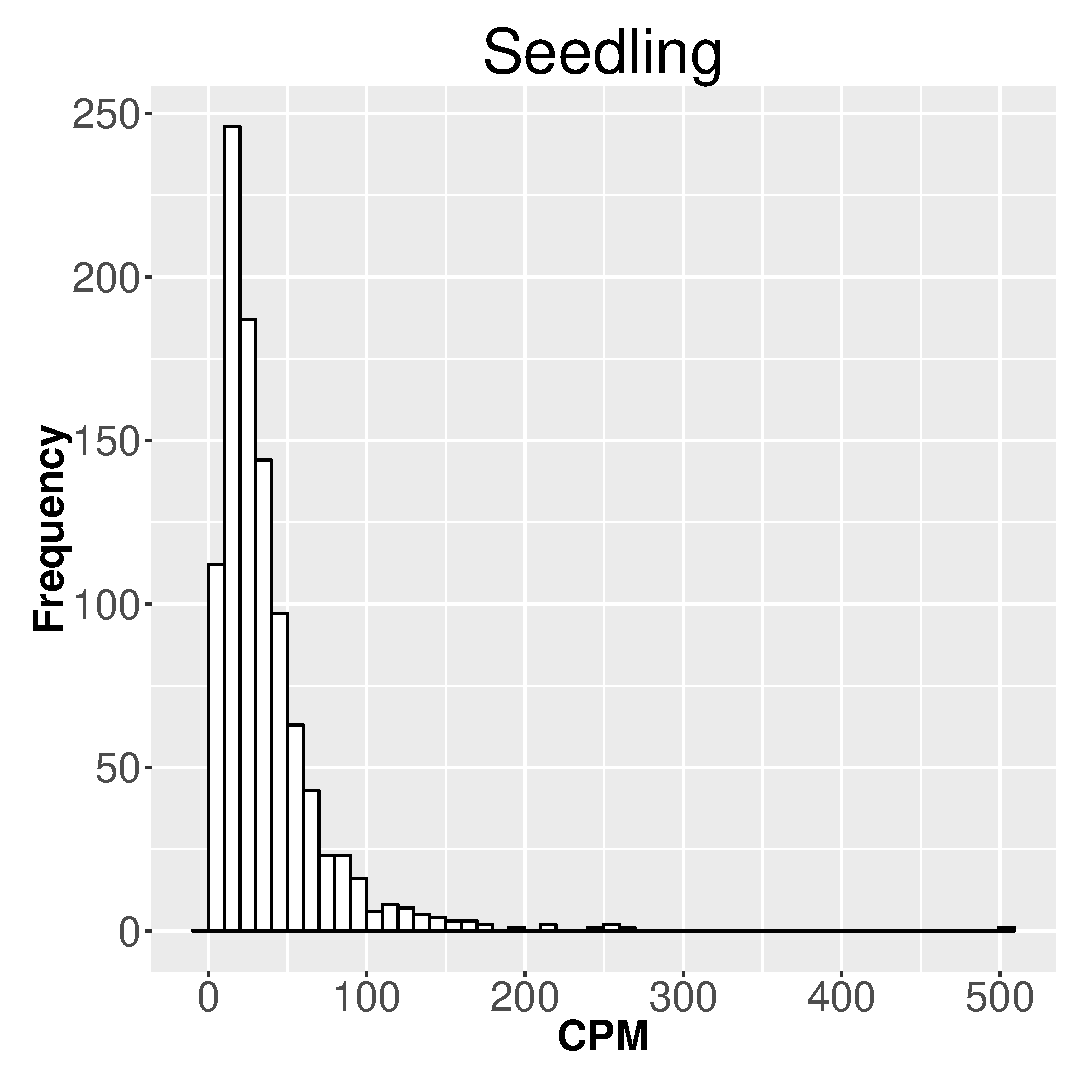
\includegraphics[width=4.5cm,height=4cm]{Figures/cpm_seedling.eps}
	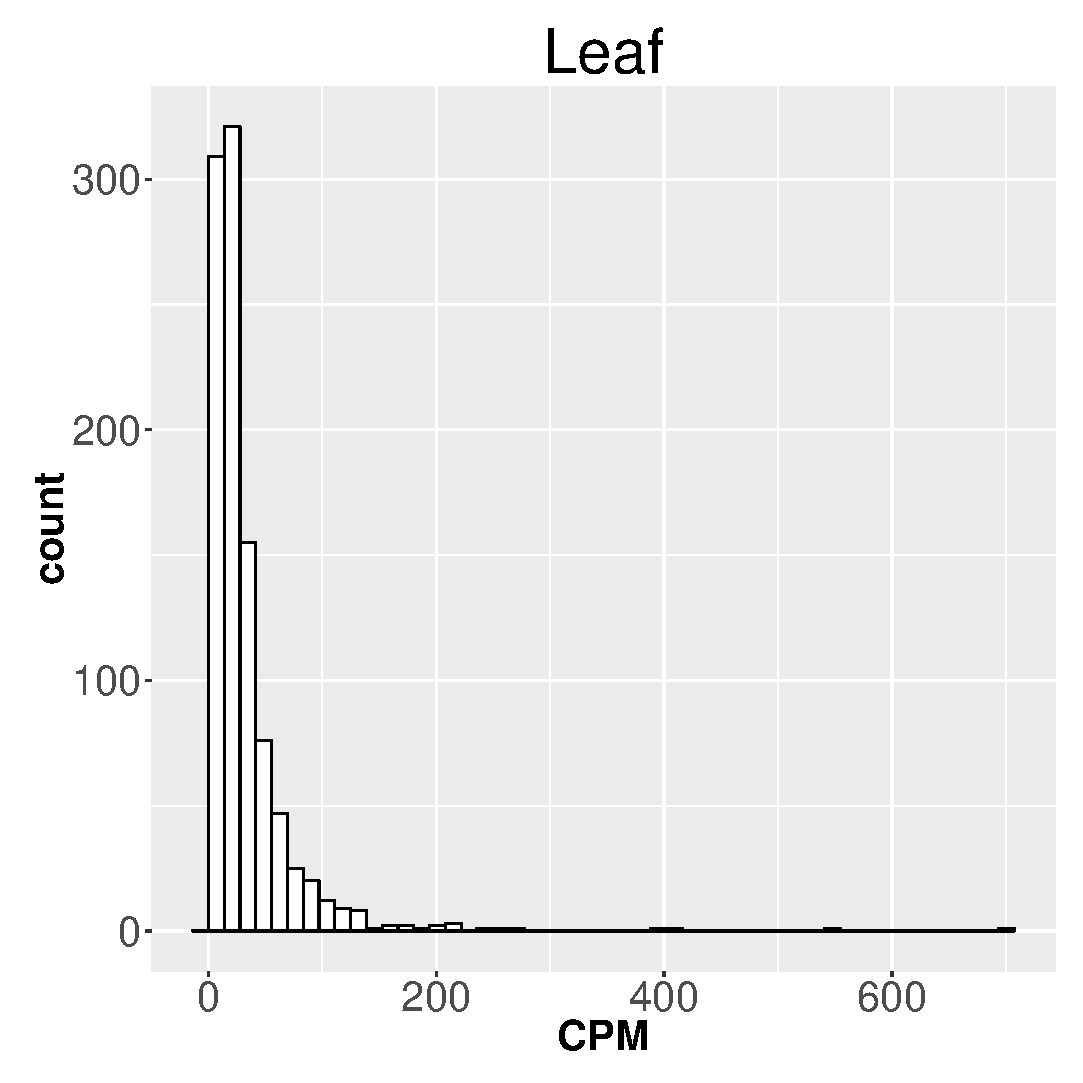
\includegraphics[width=4.5cm,height=4cm]{Figures/cpm_leaves.eps}
    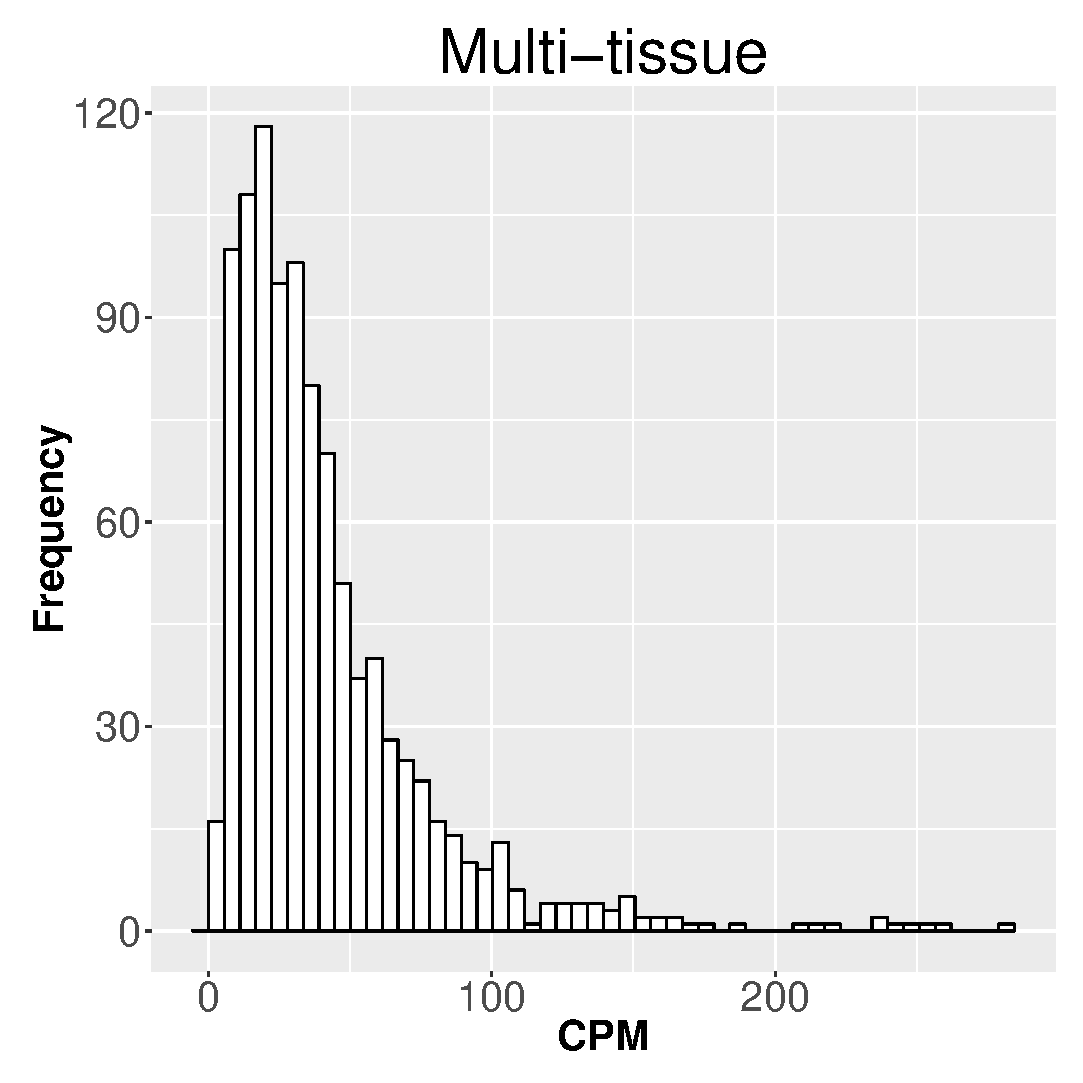
\includegraphics[width=4.5cm,height=4cm]{Figures/cpm_tissue.eps}
    \caption{{\small{\label{cpm} 
    Histograms of the mean CPM (see equation (\ref{eq:cpm})) for the top 1000
    most stably expressed genes identified from the seedling (left), leaf (middle) and multi-tissue
    (right) groups
    using  the total variance measure $\hat{\sigma}^2$}}. 
    The mean CPM is computed over all samples within each respective group. Note that the $x$ and $y$ axis scales differ between the three plots.
    } \end{center} 
\end{figure} 

% The mean CPM  of top 1000 genes, each averaged across all samples, vary from
% 2.0 to 499.0 for seedling, from 0.2 to 693.4 for leaves, and 0.4 to 278.8,
% constituting a broad range of expression values.

The lists of the top 1000 genes in the three groups share \overlapGene genes in common (see supplementary material for details).  These
genes are stably expressed under a wide range of experimental conditions and
in different tissue types, and thus may be worth further study. This list of
\overlapGene genes has significant overlap with the top $100$ stably expressed genes
identified by \cite{czechowski2005genome} from a developmental series of
microarray samples: \overlapGeneCze out of these \overlapGene genes (see Table 4 in the
supplementary material for details),
\begin{center}
\begin{quote}
%	AT5G46630, AT4G24550, AT1G13320, AT5G26760, AT1G10430, \\
%	AT4G27120, AT3G01150, AT3G10330, AT4G32560, AT2G20790, \\
%	AT1G10430, AT1G13320, AT1G54080, AT2G20790, \\
%	AT2G32170, AT3G10330, AT4G24550, AT4G27120 \\
AT1G13320, AT1G54080, AT2G20790, AT2G32170, AT3G10330,\\
 AT4G24550, AT5G26760, AT5G46210, AT5G46630, \\
\end{quote}
\end{center}
appeared in the list of the top $100$ stably expressed genes
out of $14000$ genes they examined (the probability is \overlapProb for
a list of \overlapGene genes random selected from a set of $14000$ genes to have an
overlap of size \overlapGeneCze or more with a pre-selected list of $100$ genes). In
particular, one gene, AT1G13320, is in all but one of the ten lists of top 500 stably
expressed genes identified by \cite{czechowski2005genome} for different
experimental and experimental conditions (the only exception is the set of
diurnal series), and is also identified by
\cite{hong2010identification} as a stably expressed gene under all but one of the six
experimental conditions they examined.  This gene is ranked \rankInSeedling (top \rankTopPctSeedling), \rankInLeaf
(top \rankTopPctLeaf), \rankInTissue (top \rankTopPctTissue) in the three
groups we examined, respectively, according to our stability measure.
This gene is a subunit of protein phosphatase type 2A complex and is involved in
regulation of phosphorylation and regulation of protein phosphatase type 2A
activity. It has been used as a reference gene for normalization in many
papers (e.g., \cite{bournier2013arabidopsis}, \cite{baron2012transcriptional};
these two papers cited \cite{czechowski2005genome} as reference). 

% (Similar genes are AT1G10430, AT3G01150, [AT5G46630, encoded proteins involved in adaptor complex subunits of claturin which mainly involved the protein transport and cell division process]


\subsection{Comparison to house-keeping genes and stably expressed genes
identified from microarray data}\label{section:CompareStablyExpressedGene}
\cite{czechowski2005genome} discussed the expression stability of
house-keeping genes and showed that the house-keeping genes are not stably
expressed according to their numerical measure. In particular, they compared
the expression profiles of five traditional house-keeping genes (AT1G13440,
AT3G18780, AT4G05320, AT5G12250, AT5G60390) and five genes (AT1G13320,
AT5G59830, AT2G28390, AT4G33380 and AT4G34270) that they identified  as stably
expressed according to the CV measure from a developmental series of
microarray experiments (see Figure 1 of that paper).  
In Figure \ref{expressionlevel1}, we compare the expression profiles 
of these 10 genes from \cite{czechowski2005genome} to the expression profiles
of five genes (\SelectFiveGene) that we
randomly selected from the top 100 most stably expressed genes identified from
the multi-tissue group RNA-Seq data according the total variance $\hat\sigma^2$.
For each of the 15 genes, Figure \ref{expressionlevel1} shows the expression levels measured
in CPM over \howmanytissuesample samples in the eight experiments in the multi-tissue group,
and Table \ref{table:15genes} summarizes the variance components estimated from the
GLMM in \ref{subsection:OurMethod}. 

\begin{figure}[htbp]
    \begin{center}
	\begin{tabular}{c}
	    (a)\\
	    \includegraphics[width=14cm,height=6cm]{Figures/glmm.eps} \\
	    (b) \\
	    \includegraphics[width=14cm,height=6cm]{Figures/czechowski.eps} \\
	    (c) \\
	    \includegraphics[width=14cm,height=6cm]{Figures/hkg.eps}
	\end{tabular}

	\caption{Expression profiles of 15 genes---as measured by RNA-Seq CPM---across \howmanytissuesample
	samples in the multi-tissue group. The 15 genes include (from top to
	bottom) a) five stably expressed genes (randomly selected out of the top 100)
	identified from the multi-tissue group RNA-Seq data using the total variance measure $\hat{\sigma}^2$, b) five stably
	expressed identified by \citet{czechowski2005genome} according to the CV measure from a
	developmental series of microarray experiments, and c) five
	traditional house-keeping genes (HKG) discussed in
	\citet{czechowski2005genome}. 
	}
	\label{expressionlevel1}
	%	\caption{{\small{\label{expressionlevel1} CPM of 15 genes for each sample in the multi-tissue group:  five stably expressed genes identified by the total variance $\hat{\sigma}^2$ (top), five stably expressed identified by Czechowski according to the CV measure from a developmental series of microarray experiments (middle), and  five traditional house-keeping genes (bottom).}}
    \end{center}
\end{figure} 

% Please add the following required packages to your document preamble:
% \usepackage{multirow}
\begin{table}[]
	\centering
	\caption{Variance components estimated from the multi-tissue group
	RNA-Seq data for the 15 genes in Figure~\ref{expressionlevel1}
	(identified from different sources).
	Columns 3--5 are the estimated
	variance components. Column 6 lists the stability ranking according to the
	total variance $\hat{\sigma}^2$ in the multi-tissue group.}
	\label{table:15genes}
	\begin{tabular}{rp{2cm}p{2cm}p{2cm}p{2cm}rp{1cm}}\\ \hline
		Source                        & Gene      & betweeen-sample & between-treatment & between-experiment & Rank  \\  \hline
		\multirow{5}{*}{RNA-Seq}   
		 & AT1G75420 & 0.0012 & 0.0014 & 0.0050 & 5 \\ 
		  & AT5G48340 & 0.0042 & 0.0019 & 0.0074 & 46 \\ 
		  & AT2G32910 & 0.0007 & 0.0019 & 0.0113 & 53 \\ 
		  & AT1G64840 & 0.0051 & 0.0008 & 0.0095 & 72 \\ 
		  & AT3G51310 & 0.0028 & 0.0025 & 0.0100 & 73 \\ \hline
	 
	\multirow{5}{*}{Microarray}  & AT2G28390 & 0.0034 & 0.0000 & 0.0111 & 62 \\ 
			   & AT1G13320 & 0.0036 & 0.0003 & 0.0258 & 513 \\ 
				& AT4G34270 & 0.0063 & 0.0000 & 0.0365 & 1074 \\ 
				 & AT1G59830 & 0.0044 & 0.0039 & 0.0370 & 1211 \\ 
				 & AT4G33380 & 0.0103 & 0.0016 & 0.0747 & 3404 \\ \hline
				 
	 \multirow{5}{*}{HKG}    & AT1G13440 & 0.0234 & 0.0058 & 0.1375 & 6562 \\ 
		 & AT5G60390 & 0.0267 & 0.0068 & 0.2270 & 8867 \\ 
		 & AT4G05320 & 0.0123 & 0.0094 & 0.2690 & 9409 \\ 
		 & AT5G12250 & 0.0313 & 0.0128 & 0.3262 & 10589 \\ 
		 & AT3G18780 & 0.0375 & 0.0211 & 1.0313 & 14951 \\ \hline 
	\end{tabular}
\end{table}

% also, Czechowski's reference genes are
% relatively more stable (middle); furthermore, we identified a set of genes
% with even higher expression stability (bottom).

The five house-keeping genes show large total variation with all three
variance-components relatively large as compared to the other 10 genes. This is
consistent with Czechowski's observation that house-keeping genes are not necessarily stably
expressed according to a numerical measure. Three of the five
stably-expressed genes identified by Czechowski are among the top $1000$
stably-expressed genes according to our stability measure, the total variance $\hat\sigma^2$. Czechowski et al.
identified those five genes from microarray data and different experiments. It
is not too surprising those genes might not be the most stable in RNA-Seq
experiments: the two technologies differ in many aspects including coverage
and sensitivity. 


% \subsection{Comparison of different stability measures}\label{section:stabilityMeasure}
\subsection{Factors affecting stability ranking}\label{section:stabilityMeasure}
The previous two subsections demonstrate that when using a numerical measure
to quantify gene expression stability, the outcome is dependent on 1) the
biological context reflected in the reference sample set used and 2) the
technology used for measuring gene expression. It should also be intuitive,
and we will further clarify in the second half of this subsection, 
that the stability ranking is also dependent on 3) the specific numerical measure used.
In this section, we will first compare the lists of stably-expressed genes
identified under different scenarios where one or more of the above three
factors differ.  We then further discuss the subtle roles played by the
specific stability measure and the reference gene set by comparing the total
variance $\hat\sigma^2$ measure from the GLMM (see equation (\ref{eq:GLMM}))
to the $M$-value measure used in the geNorm method \citep{vandesompele2002accurate}.
Last, we discuss the effect of an iterative elimination procedure used by
geNorm.

We look at an additional five lists of stably expressed genes identified under
different scenarios and examine how each of these five lists overlaps with the
the top stably-expressed genes identified from the multi-tissue group  of
RNA-Seq experiments  according to the total variance measure $\hat\sigma^2$
(see Section~\ref{subsection:OurMethod}). 
The five lists are: 
\begin{enumerate}\label{list:L5}
    \item[$L_1$:]
 100 top stably expressed genes from the multi-tissue group according
 to the $M$-value in geNorm (applied to $(\text{count}+1)$) of \cite{vandesompele2002accurate} ; 
\item[$L_2$:]	
100 top stably expressed genes from the seedling group according to the total variance $\hat\sigma^2$ from the GLMM;
\item[$L_3$:]
100 top stably expressed genes from the leaf group according to the total variance $\hat\sigma^2$ from the GLMM; 
\item[$L_4$:]
100 stably expressed genes identified from a developmental series of microarray
experiments by \cite{czechowski2005genome} using the CV measure (see Section \ref{subsection:OtherStabilityMeasure}); 
\item[$L_5$:] 50 stably expressed genes identified by \cite{dekkers2012identification} from microarray
seed experiments using the CV measure.  
\end{enumerate}
For each list $L_i$ above, we measure how it overlaps with the top stably
expressed genes (the reference set) from the multi-tissue group using the {\em
recall percentage}
\begin{equation}\label{eq:recall}
\frac{ \# \{L_i \cap \text{reference set} \}}{\# \{L_i\}}\times 100,
\end{equation}
where $\#\{ \}$ denotes the number of elements in the list. 
In Figure \ref{fig:rankVSrank_RNA}, we plot the recall percentage versus
the number of top stably-expressed genes we selected as reference from the
multi-tissue group. 

We have the following observations:
\begin{enumerate}
    \item
	The list $L_1$ is identified from the same set of RNA-Seq experiments as the
	reference sets, but using a different stability measure ($M$-value in
	geNorm). This list has significant overlap with the top
	stably-expressed genes identified using the total variance measure:
	\recalltophundred and \recalltopthousand out of the $100$ genes from the list $L_1$ are among the
	top $100$ and $1000$ most stably-expressed genes, respectively, from the
	multi-tissue group identified using the total variance measure. 
    \item
	The lists $L_2$ and $L_3$ are identified from different sets of
	RNA-Seq experiments (leaf and seedling experiments) using the same
	stability measure as used for the reference sets. The lists $L_4$ and $L_5$ are
	identified from microarray experiments (a developmental series and a
	seed group) and using the CV measure. The overlapping (recall)
	percentages are still statistically significant, but much less than in
	the case of $L_1$.  This shows that differences in tissue type and in
	measuring technology both influence the expression stability ranking,
	and to comparable degrees. The lists $L_3$ and $L_5$ have the least
	overlapping percentages with the reference sets. These lists are
	identified from a leaf group and a seed group respectively.
	Our understanding is that the leaf group and the seed group are more
	biologically homogeneous than the multi-tissue group and thus provide
	very different biological contexts for evaluating expression stability.
\end{enumerate}

%(\textbf{use stably expressed genes from RNA-Seq study when studying RNA-Seqdata!, even if not the same tissue type}) Next, we compared the consistencybetween stably expressed genes identified from seedling, leaf and multi-tissue in this study. Figure \ref{fig:rankVSrank_RNA} shows that stably expressed genes from RNA-Seq study are slightly more consistent than when comparing those from RNA-Seq data with those from microarray data, but less consistent than stably expressed genes identified from the same data with different stability measures.

%\textbf{Difference due to data sources}\\ Stably expressed genes may also vary due to different data sources. For those most stably expressed genes (top 100 in Czechowski et. al. and top 50 in Dekkers et. al., identified as stable from microarray data), only $< 40\%$ are present in top 1000 list from RNA-Seq data based on our stability measure (figure \ref{fig:rankVSrank_RNA}).

%\textbf{Difference due to biological functions}\\
% In pre-genomic era, HKGs are often believed to be stably expressed for biological reasons. HKGs are typically constitutive genes that maintain basic cellular function, and therefore are expected to express at relatively constant levels in non-pathological situations. However, stability in terms of biological functionality does not imply stability in terms of numerical expression values.  The data-driven methods are generally more reliable, as shown by various PCR validation experiments of microarray (\cite{czechowski2005genome} \cite{hruz2011refgenes}).

\begin{figure}[h!]
    \begin{center}
	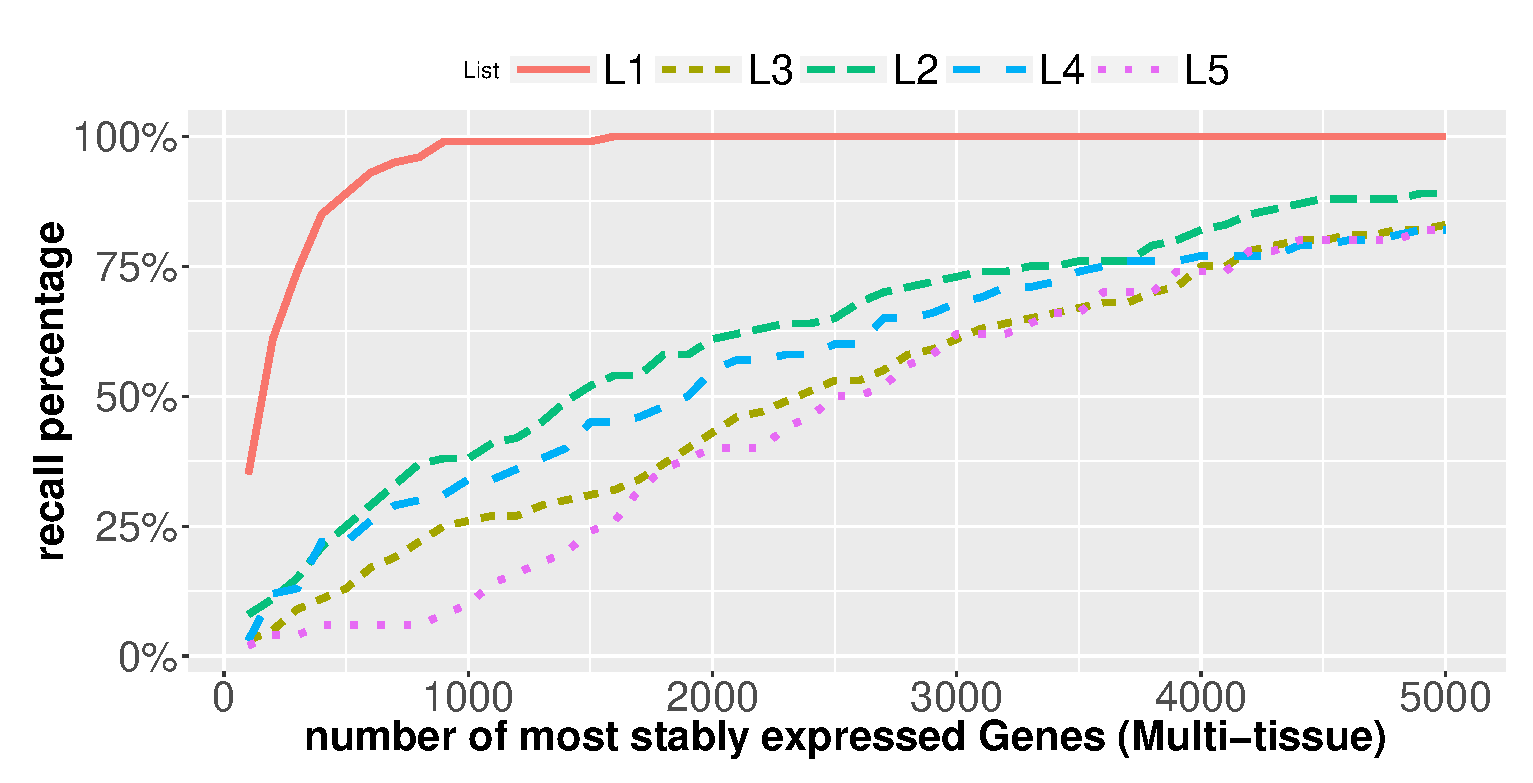
\includegraphics[scale=0.55]{Figures/rankVSrank_RNA2.eps}
	\caption{Comparison of top stably expressed genes identified under different scenarios.
	We choose the top 100 stably expressed genes as described in $L_1$--$L_4$,
	and the top 50 stably expressed genes in $L_5$ (see Section \ref{list:L5}). 
	and plot the recall percentages between these lists and the top most
	stably expressed genes identified from the  multi-tissue group
	according to the total variance measure.
	The $x$-axis is the number of most stably expressed genes in multi-tissue
	group according to the total variance measure, and the $y$-axis shows the
	recall percentage (see equation (\ref{eq:recall}))  for each of the
	five lists.}
	\label{fig:rankVSrank_RNA}
    \end{center}
\end{figure}

When applied to the same set of samples, the $M$-value and total variance
measure $\hat\sigma^2$ give similar expression stability ranking: the rank
correlation is \recallrankcorrelation (see also, observation 1 above).
% there is significant overlap between the sets of most stably-expressed genes identified
% according to the $M$-value measure and according to the total variance
% measure $\hat\sigma^2$$
% This should come as no surprise because 
We point out that the reason is because the $M$-value and normalization step
needed for computing our total variance measure have similar fundamental
assumptions. 
The basic principle
behind the $M$-value is that the expression ratio of two stably-expressed
genes should be identical in all samples. In formula, it means that the
expression values of two stably-expressed genes $i_1$, $i_2$ in any two samples $j_1$, $j_2$
should satisfy
\begin{equation}\label{eq:typical}
   \dfrac{y_{i_1, j_1}}{y_{i_2, j_1}} = \dfrac{y_{i_1, j_2}}{y_{i_2, j_2}}.
\end{equation} 
% (In practice, genes  with the more ``typical'' expression profiles are considered as more stable.)
Our total variance measure $\hat\sigma^2$ is estimated from normalized data.
The basic assumption in the normalization step is that majority of genes are
not DE. In formula, it means for any stably-expressed gene $i_1$, its expression
level as measured by the relative frequency should be stable across all
samples,
\begin{equation}\label{eq:DESeq} 
    \frac{y_{i_1, j_1}}{S_{j_1}}= \dfrac{y_{i_1, j_2}}{S_{j_2}},
\end{equation}
where $S_{j_1}$ to $S_{j_2}$ are the normalized library sizes (i.e., $R_j N_j$ in equation (\ref{eq:GLMM})).
This implies for any two stably-expressed genes $i_1$ and $i_2$
\begin{equation}\label{eq:DESeq2} 
    \frac{y_{i_1, j_1}}{y_{i_1, j_2}} = \frac{y_{i_2, j_1}}{y_{i_2, j_2}} =
    \frac{S_{j_1}}{S_{j_2}}.
\end{equation}
The first equation in (\ref{eq:DESeq2}) is equivalent to equation
(\ref{eq:typical}). (In practical application of both methods, the stability
of any single gene is evaluated by comparing its expression to a set of
reference genes. See the Method section \ref{section:countNormalization} for more details.)

In practice, the geNorm program \citep{vandesompele2002accurate} is frequently
used to rank a set of reference genes identified from other methods.  An
iterative elimination procedure is used along with the $M$-value to determine
the final ranks of the expression stability:  after each iteration, the gene
receiving the largest $M$-value will be removed and a new set of $M$-values
will be computed for the remaining genes, and the iteration will go on until
there are only two genes left.  We did not use such an iterative procedure in
the comparisons above (i.e., we only computed one set of $M$-values for all
genes). 

This iterative elimination procedure creates an extra layer of complexity that
is not well explored in literature. We use a toy example below to illustrate
one subtle aspect of the iterative elimination procedure.  In this example, we
consider the expression values of 7 genes in two samples shown in Table
\ref{table:toyexample}. When $M$-value is used to rank all $7$ genes, the
initial ranking of expression stability is given in column 4 of the table:
gene $7$ is the least stable and genes $4$ and $5$ are considered the most
stable ones.  Once genes 6 and 7 are eliminated, however, the recalculated
$M$-values will rank genes 1--3 as more stable than genes $4$ and
$5$ (see column 5 of Table \ref{table:toyexample}). The root cause of this
reversal of ranking is that when an iterative elimination procedure is used,
effectively, the reference gene set is changing after each iteration: in the
initial ranking, the expression patterns genes 4 and 5 are close to the
``middle of the pack'' and thus considered as the most stable, and the
expression patterns of genes 1--3 and genes 6 and 7 are considered relatively
more extreme; once genes 6 and 7 are removed, however, the ``middle of the
pack'' is shifted towards the expression patterns of genes 1--3, and thus
genes 1--3 become the most stably expressed.  With this understanding, one
could and should make a conscious decision on whether such a behavior as
described above is desirable or not.  

The point we want to emphasize is that gene stability is a relative concept
and the stability ranking depends on which set of genes we use as reference.
In an iterative elimination procedure, the reference gene set will change
after each iteration. The procedure can thus give surprising results and the
adoption of it in practice should not be automatic.

 
\begin{table}[ht] \centering \caption{A toy example showing the effect of
    iterative elimination. Columns 2 and 3 represent expression levels for
    seven genes in two samples, column 4 is the stability ranking of genes by
    $M$-value without iterative elimination, and column 5 is the ranking after
    two geNorm iterations.} 
	\begin{tabular}{rrp{2cm}rp{2cm}rp{2cm}rp{2cm}}
    \hline & \multicolumn{2}{c}{Raw Counts} & \multicolumn{2}{c}{Rank}\\
     Gene & sample 1 & sample 2 & rank 1 & rank 2 \\ \hline 
    Gene1 & 1 & 1 & 3 & 1 \\ 
    Gene2 & 1 & 1 & 3 & 1 \\ 
    Gene3 & 1 & 1 & 3 & 1 \\
     Gene4 & 1 & 2 & 1 & 4 \\ 
     Gene5 & 1 & 2 & 1 & 4 \\ 
     Gene6 & 1 & 3 & 6 &  \\ 
    Gene7 & 1 & 4 & 7 &  \\ \hline 
    Library Size & 7 & 14 & & 	\\ \hline 

  %  Note: &\multicolumn{4}{l}{ rank1 = initial ranking by $M$-value, } \\
%    & \multicolumn{4}{l}{ rank2= ranking after genes 6 and 7 removed.}
\end{tabular} \label{table:toyexample} \end{table}




%With the same RNA-Seq data, we identified top 1000 stably expressed genes for both geNorm and NormFinder algorithms. There is substantial consistency (Figure \ref{fig:wenn}) between different stability measures. For example, the agreement between geNorm and our method suggests that the most typical expression pattern is stable expression (i.e., has low variance in the estimated log relative mean of normalized counts). 

%\begin{figure}
%\centering
%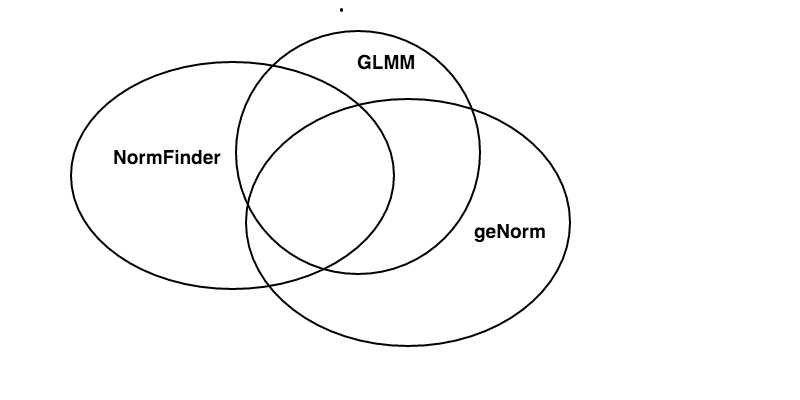
\includegraphics[width=0.7\linewidth]{Figures/wenn.eps}
%\caption{Overlap diagram: each circle represents top 1000 stably expressed genes from geNorm, NormFinder and our method}
%\label{fig:wenn}
%\end{figure}


\subsection{Sources of variation}\label{Section:varianceComp}

For each gene, the GLMM (equation (\ref{eq:GLMM}) of section
\ref{subsection:OurMethod}) allows us to decompose total count variance into
between-sample, between-treatment and between-experiment variance components.
The estimated variance components tell us how much each component contributes
to the overall count variation. Table \ref{table:percentageofvariation}
summarizes the percentages---averaged over all genes---of the total variance
attributable to each of the three components for three groups of RNA-Seq
samples (seedling, leaf and multi-tissue groups in Section
\ref{section:DataCollection}). Figure \ref{fig:densityplot} shows the
histograms of the percentages.  Figure \ref{fig:all} shows the stacked bar
plot of variance components estimated from the multi-tissue group for 20 genes
randomly selected from the top 1000 stably expressed genes and 20 genes
randomly selected from 23611 genes.  As expected, the between-experiment
variance component, on average, explains the largest proportion of the total
variation. The between-experiment variation is relatively smaller among the
leaf samples, indicating that the leaf samples are more homogeneous.  There is
more variation in the relative percentages of total variance explained by the
between-sample and between-treatment variance components. In principle, the
between-treatment variation will be greater when there is a higher proportion
of DE genes or when the samples are more homogeneous. In practice, the
between-sample variance depends greatly on what samples are used as biological
replicates. 

%The between-experiment variation, on average, is largest in the multi-tissue group
% One implication is that DE is easier to detect in
%this group of experiments.  
%Our intuition is that leaf samples tend
%to be more homogeneous and thus the treatment effect is easier to detect
%between leaf samples.
%
%
%In the group of leaf
%experiments, the between-treatment variation is markedly greater than the
%between-sample variation, suggesting the existence of a higher proportion of DE genes.
%%The between-experiment variation, on average, is largest in the multi-tissue group
%One implication is that DE is easier to detect in
%this group of experiments.  
%Our intuition is that leaf samples tend
%to be more homogeneous and thus the treatment effect is easier to detect
%between leaf samples.
%
%([Ask Jeff], one implication is that DE is easier to detect in
%this group of experiments.  
% Our intuition is that leaf samples tend
%to be more homogeneous and thus the treatment effect is easier to detect
%between leaf samples. ) 
 
\begin{center} 
     \begin{table}[!ht] 
	 \centering 
	 \caption{Percentages---averaged over all genes---of the total
	 variance attributable to each of the three variance components
	 (between-sample, between-treatment, between-experiment) for the three
	 groups of RNA-Seq samples (the seedling, the leaf and the
	 multi-tissue groups). %The variance components were estimated by fitting the GLMM model to the samples in the respective group.
	 } 
	 \label{table:percentageofvariation}

     \begin{tabular}{lp{3cm}p{2.5cm}p{3cm}}\hline
     Source & Seedling & Leaf & Multi-tissue \\  \hline
		between-sample & 7.2\% & 16.0\% & 7.6\% \\ 
		between-treatment & 20.1\% & 28.0\% & 5.1\% \\ 
		between-experiment & 72.6\% & 56.0\% & 87.3\% \\ \hline
     \end{tabular} \end{table} \end{center}

 \begin{figure}[!ht]
\begin{center}
\includegraphics[width=14cm,height=1.5cm]{Figures/var_dens_legend.eps}
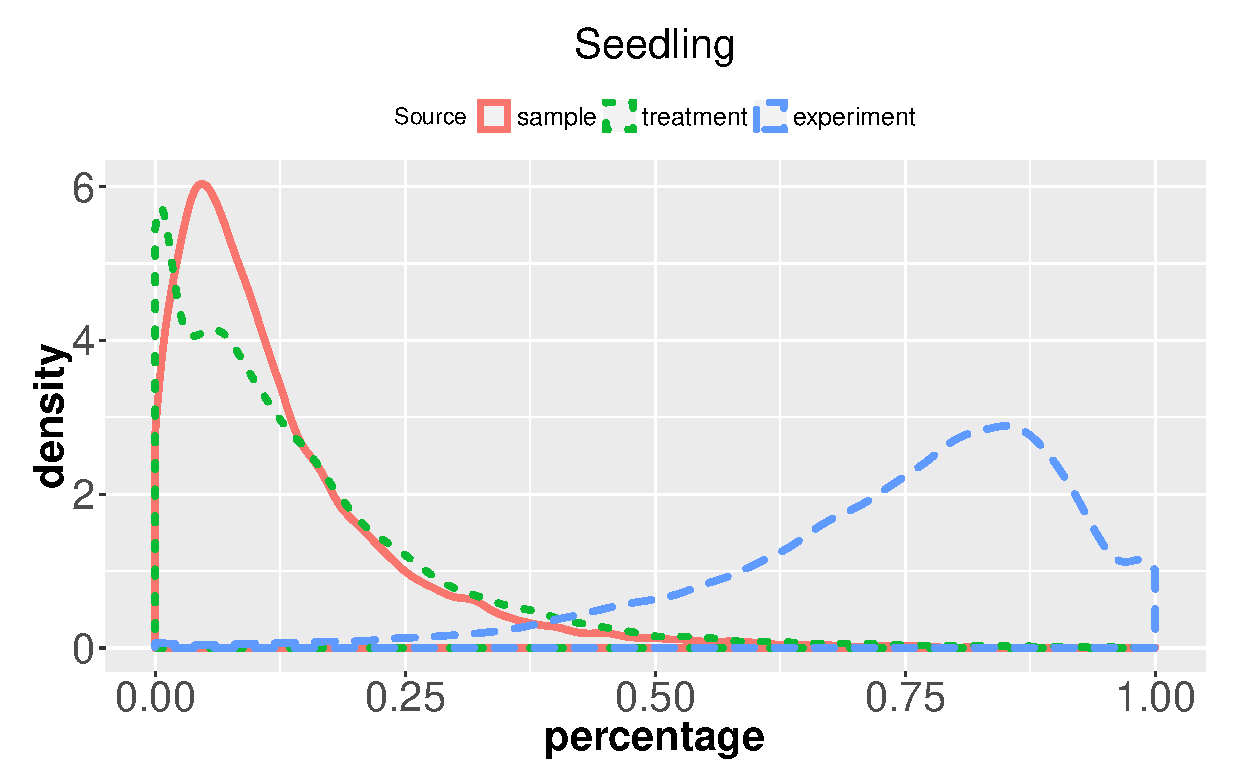
\includegraphics[width=4.5cm,height=4cm]{Figures/var_dens1.eps}
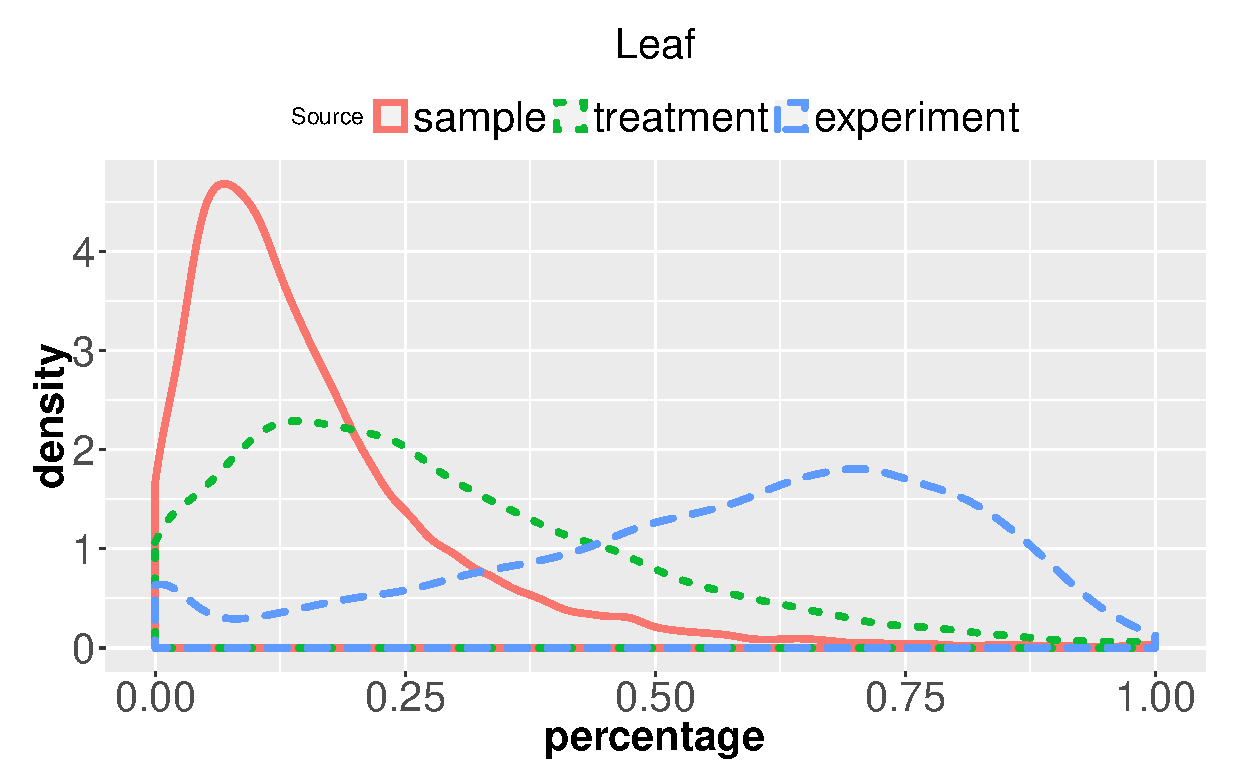
\includegraphics[width=4.5cm,height=4cm]{Figures/var_dens2.eps}
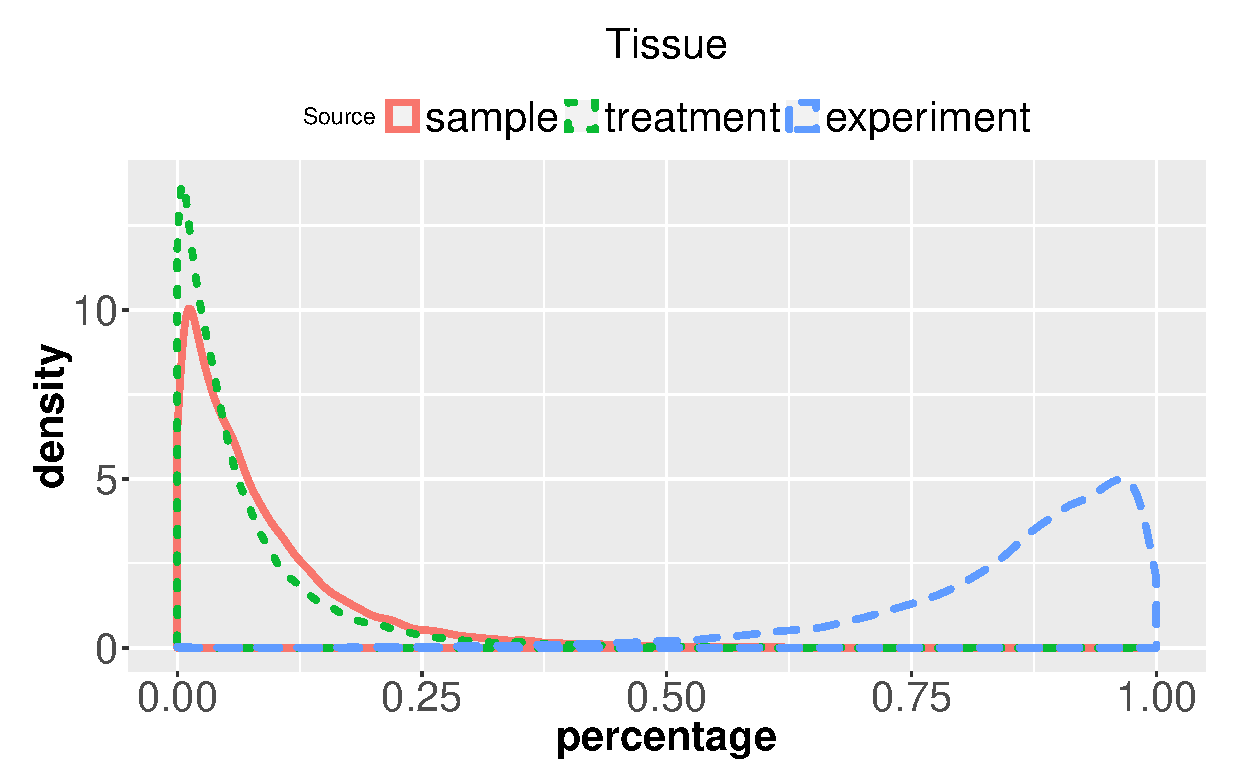
\includegraphics[width=4.5cm,height=4cm]{Figures/var_dens3.eps}
\caption{Distributions (over all genes) of the percentages of the total
variance attributable to the between-sample, and between-treatment, or the
between-experiment variance component, in the seedling, the leaf, and the
multi-tissue groups.}
\label{fig:densityplot}
\end{center}
\end{figure} 


\begin{figure}[!ht]
	\centering
	%\includegraphics[width=15cm, height= 1.5cm]{Figures/stackbar_legend.eps}
	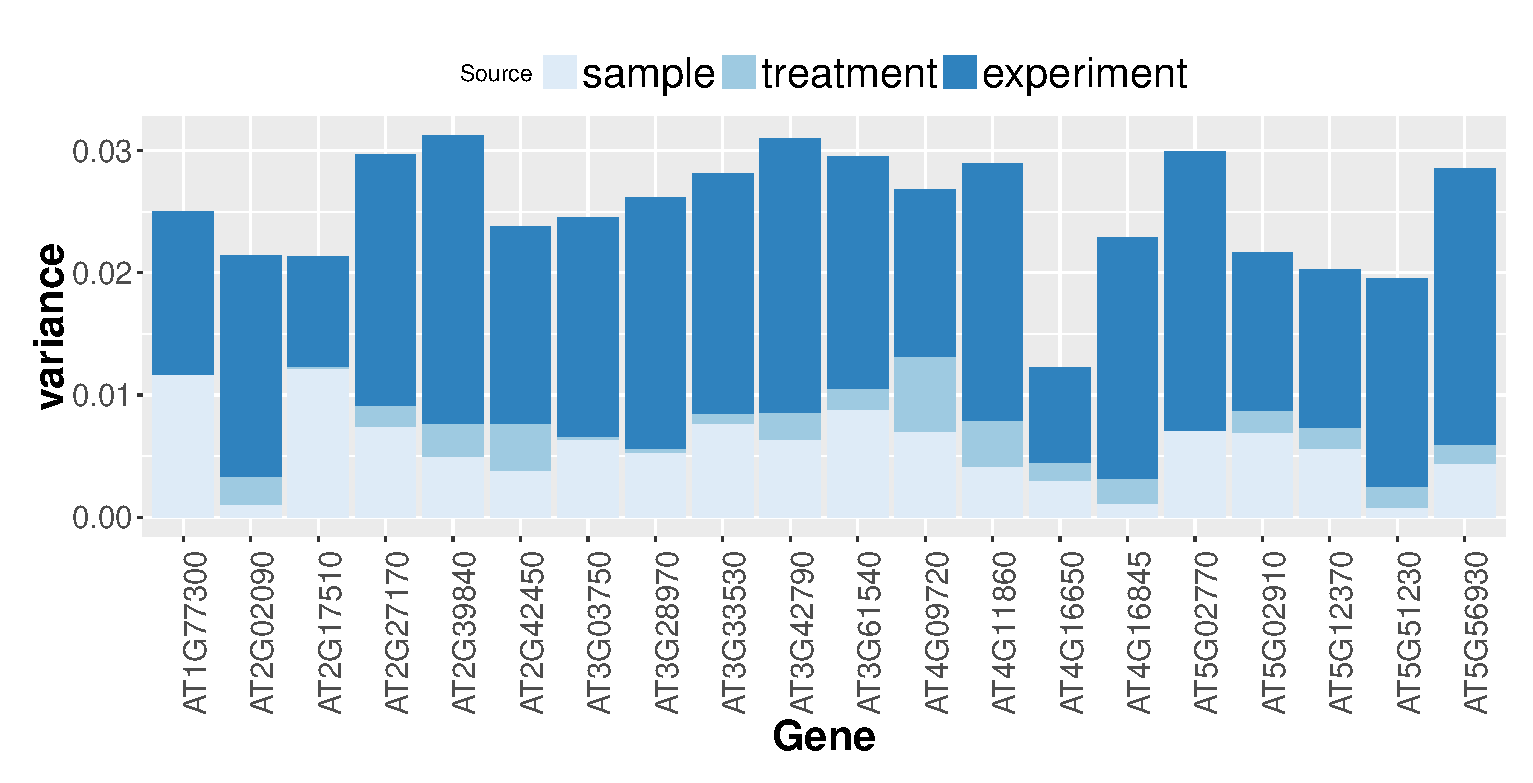
\includegraphics[width=14cm, height= 7cm]{Figures/top1000.eps}
	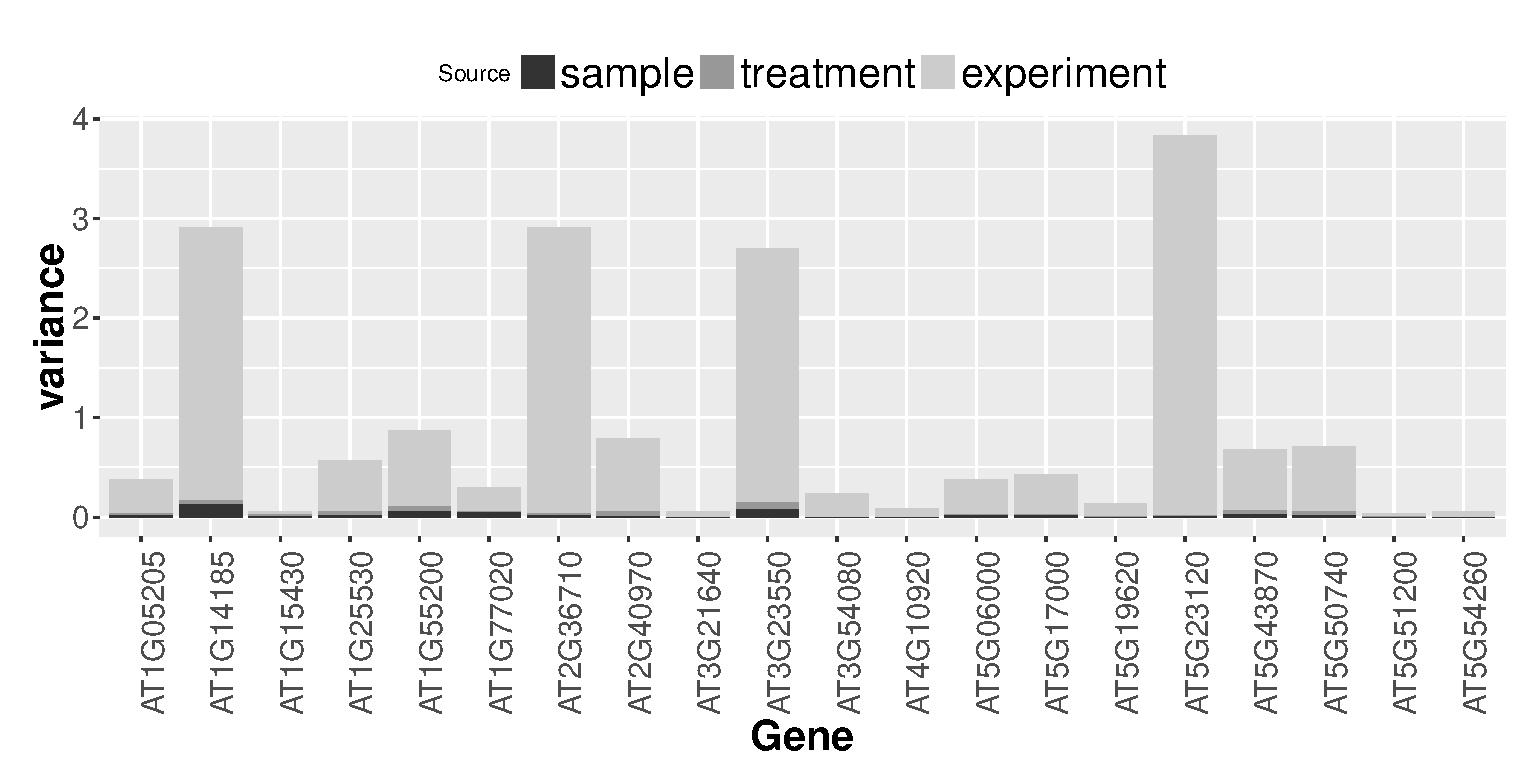
\includegraphics[width=14cm, height= 7cm]{Figures/all.eps}
	\caption{Stacked bar plots of the three variance components for
	selected genes in the multi-tissue group. Top: 20 genes randomly selected from top 1000 stably expressed genes; Bottom: 20 genes randomly selected from all the genes.}
	\label{fig:all}
\end{figure}


\subsection{Reference gene set for normalization}
\label{Section:commonReference}

Once we have ranked the genes according to our numerical stability measure
(i.e, the total variance measure, $\hat\sigma^2$), one application is to use
an explicit set of most stably expressed genes as reference genes for count
normalization.  This new approach allows investigators to prescribe a specific
biological context for evaluating gene stability by choosing the most relevant
reference samples and experiments when computing the stability measure.  For
example, the most stably expressed genes identified from the multi-tissue
group and those identified from the seedling group will provide different
biological contexts. In contrast, existing normalization approaches are often
applied to the single data set under study, and thus provide a single, narrow
context.

% We can think the differences between the two approaches as using external
% control set and using an internal control set.

Even under a specific biological context,  it is almost impossible to know
whether the genes in any reference set are absolutely stably expressed, even
though commonly used normalization methods often enforce some assumptions on
the reference gene set: for example, when we use Anders and Huber's
method to estimate the normalization factors based on a subset of reference
genes, roughly speaking, the median fold change among the reference genes will
be set to 1 (see Section \ref{section:countNormalization} for more details). A
subtle point we want to make is that since it is impossible to know how well
such or similar assumptions on DE hold for a reference gene set,
% to be useful as a reference set: 
we can improve the interpretability of the DE test results by making the
reference gene set explicit:  we can slightly change our perspective and
interpret all DE results as relative to the reference gene set.  
% a reference gene set does not have to be absolutely stably expressed to be
% useful as a reference set: 
For example, a fold change of 2 inferred from the GLMM model can be
interpreted as the fold change of a gene is 2 times the true (but often
unknowable) median fold change of the reference genes.  
% Strictly, the normalization is performed at the sample level. This statement is
% about median fold change between two groups.
When one estimates the normalization factors based on all genes, one is
effectively specifying an implicit set of genes as a reference set.  Our
proposal is to make the reference set explicit and interpret DE results as
relative to the reference gene set.


\begin{center}
    \begin{table}\centering
	\caption{A toy example for illustrating the importance of using a
	common explicit set of reference genes when comparing RNA-Seq data from
	multiple experiments. If a common reference gene set (e.g., genes
	1--3) is used as reference for count normalization, we will notice
	that the DE behavior of gene 3 differs in the two experiments. If the
	two experiments are separately normalized using genes 1--3 as
	reference in experiment 1, but using genes 3--5 as reference in
	experiment 2, we may conclude that gene 3 is not DE in either group.
	}\label{table:reference}
	\begin{tabular}{cccccc} \hline
	    &  \multicolumn{2}{c}{Exp. 1} & & \multicolumn{2}{c}{Exp. 2} \\
	    \cline{2-3}  \cline{5-6}
	    % Gene  & $T_{1, 1}$ & $T_{1, 2}$  & $T_{2, 1}$  &$T_{2, 2}$ \\ \hline
	    Gene  & Control & Treatment & & Control & Treatmetn \\
	    \hline
	    1     & 10       & 20    &   & 10    &20   \\
	    2     & 10       & 20    &   & 10    &20   \\
	    3     & 10       & 20    &   & 10    &10   \\
	    4     & 10       & 10    &   & 10    &10   \\ 
	    5     & 10       & 10    &   & 10    &10   \\  
	    \hline
	\end{tabular}
    \end{table}
\end{center}

%	\begin{center}
%	\begin{table}\centering
%		\caption{My caption}\label{table:reference}
%		\begin{tabular}{ccccc} \\ \hline
%			&  \multicolumn{2}{c}{Exp. 1} & \multicolumn{2}{c}{Exp. 2} \\
%			Gene  & $T_{1, 1}$ & $T_{1, 2}$  & $T_{2, 1}$  &$T_{2, 2}$ \\ \hline
%			1     & 10       & 20       & 10    &20   \\
%			2     & 10       & 20       & 20    &10   \\
%			3     & 10       & 10       & 10    &10   \\
%			4     & 20       & 20       & 20    &20   \\ 
%			5     & 20       & 40       & 20    &20   \\  \hline
%			total & 70       & 110      & 80   &80   \\ \hline
%		\end{tabular}
%	\end{table}
%	\end{center}

Interpreting the DE results as relative to an explicit reference set is
especially beneficial when one wants to compare DE results from an experiment
to previously published results.
% ones that are publicly available. 
When the interest is in comparing different experiments, we recommend using a common reference set. 
% In the Introduction, we also argued that using an explicit set of genes as
% reference for normalization can improve interpretability of DE results, in the
% sense that DE can always be interpreted as relative to the explicit reference
% gene set used. 
For example, when two RNA-Seq data sets are separately
normalized with different reference sets, a fold change of two observed in one
experiment may not be directly comparable to a fold change of two observed in
the other.  This concern can be alleviated by using a common set of reference
genes.  We use a toy example to illustrate this point in Table
\ref{table:reference} where we examine the mean counts for 5 genes in two
two-group comparison experiments. If we use different reference gene sets for
 count normalization in the two experiments, for example, we use genes 1--3 as reference in experiment
1, but use genes 3--5 as reference in experiment 2, we may conclude that gene
3 is not DE in either experiment. If we use a common reference gene
set---either genes 1--3 or genes 3--5---for normalization, however, we will be
able to discover, in either case, that the DE behavior of gene 3 is different
in the two experiments. Note that the DE conclusion in both experiments will
depend on the reference genes used: if genes 1--3 are used as reference, gene
3 is not DE in experiment 1, but will be DE in experiment 2; if genes 3--5 are
used as reference, gene 3 will be considered DE in experiment 1, but not DE in
experiment 2. The point is, in either case, we will notice that the DE
behavior of gene 3 is different between the two experiments. This information
will be lost if one uses different reference sets to assess DE in the two
experiments.


% Columns 2--5 are the mean counts for each treatment. 
%In Experiment 1, expression levels of genes 1, 2, and 5 represent
%the most typical pattern and therefore they are used as reference genes; as a
%result, genes 3 and 4 will be declared as DE. In Experiment 2, expression
%levels of gene 3--5 are most typical and therefore used as reference genes,
%and genes 1 and 2 will be considered as DE. However, when comparing the two
%experiments and we use genes 3 and 4 as commen reference, genes 1 and 2 will
%be declared as DE in both experiments and gene 5 will be considered as DE in
%experiment 1 but not DE in experiment 2.
%

In practice, we recommend using the top 1000 most stably expressed genes for
estimating normalization factors. The key is to avoid using too few (e.g.,
less than 10) or too many (e.g., using all genes) reference genes:
intuitively, using too few, the estimates will be unstable; using too many,
the results may be subject to influence from highly unstable genes.
Our simple simulations suggest that using between 100 to 10000 genes seems to
give stable results. In the first set of three examples, we used Anders and
Huber's method (see equation (\ref{eq:normfactors})) to estimate normalization
factors for samples in each of the seedling, leaf and multi-tissue groups of
experiments (see Section \ref{section:DataCollection}).  We used the top 10,
100, 1000, and 10000 stably expressed genes identified earlier (see Section
\ref{section:stablyExpressedGene} for details) as reference gene sets. Figure
\ref{fig:normfactor} shows the pairwise scatter plots and correlation
coefficient between the normalization factors when different numbers of top
stable genes are used as reference. A stronger correlation indicates the
normalization factors estimated from the two settings are highly consistent.
The plots and correlation coefficients suggest using between 100 and 1000
genes tend to give similar normalization factor estimates. We also used the
top 10, 100, 1000, and 10000 stably expressed genes identified from the
multi-tissue group as reference set for estimating normalization factors for a set
of 48 root samples from a new experiment (GSE64410, \cite{vragovic2015translatome}). The largest Pearson correlation
$0.993$ is between the normalization factors estimated using the top $100$
and top $1000$ stably expressed genes as reference. Based on the above
observations, using 1000 most stably expressed genes as reference seems to be
a reasonable heuristic rule.

%A common reference set of stably expressed genes will help improve
%comparability of the data sets and interpretability of DE test leaf.



\begin{figure}[!ht]
	\begin{center}
		\includegraphics[scale=0.34]{Figures/norm_seedling.eps}
		\includegraphics[scale=0.34]{Figures/norm_leaf.eps}
		\includegraphics[scale=0.34]{Figures/norm_tissue.eps}
		\includegraphics[scale=0.34]{Figures/norm_GSE64410.eps}
		\caption{Matrices of scatter plots of normalization factors
		estimated using different reference gene sets. 
		The upper-left, upper-right and lower-left plots show
		normalization factors estimated for the samples in the
		seedling, leaf, and multi-tissue groups correspondingly. 
		In each case, the top 10, 100, 1000, and 10,000 stably
		expressed genes are used as reference to
		calculate the normalization factors.
		The lower right plot shows the normalization factors estimated for a new root
		experiment (GSE64410, with sample size 48) using the top 10--10,000
		stably expressed genes identified from the multi-tissue group as
		reference. The normalization factors are estimated using the
		method described in Section \ref{section:countNormalization}.}
		\label{fig:normfactor} \end{center} \end{figure}

  \section{Conclusion and Discussion}\label{section:discussion}
  
In this paper, we advocate quantifying gene expression stability by applying a
numerical stability measure to a large number of existing RNA-Seq data sets.
Similar strategies have also been used by others to find stably expressed
genes from microarray data. Since DE is measured by relative frequencies, we
argue that DE is a relative concept and using an explicit reference gene set
can improve interpretability of DE results, and furthermore,  using a common
reference gene set can avoid inconsistent conclusions when comparing multiple
experiments (see Section \ref{Section:commonReference}).

%We emphasize that numerical stability is not equivalent to biological
%stability (??? Jeff, about  ``biological stability'': do
%biologists talk about ``biological stability''?) For example, we demonstrated
%that the expression levels of traditional house-keeping genes are not
%necessarily stable according to a numerical measure. 
%Biological stability is a vague term and not easy to quantify.  Numerical
%stability is generally more tractable.

% (Some have argued that numerically
% somewhat circular??? The same numerical measure is used to both identify the
% stably expressed genes and to verify their stability.) 

It should be clear but worth emphasizing that when using a numerical measure
to identify stably expressed genes, the outcome depends on multiple factors:
the background sample set and the reference gene set used for count
normalization, the technology used
for measuring gene expression, and the specific numerical stability measure
used.  In this study, to illustrate our proposed methods, we identified three
sets of stably expressed genes from three sets of Arabidopsis experiments. The
major point is that stably expressed genes identified from different
backgrounds will provide different biological contexts for evaluating
differential expression. In practice, researchers can choose the specific
context. A practical challenge in applying such a philosophy is that no two
experiments will have identical settings, and researchers have to decide what
experiments can be considered comparable. This is a difficult question;
however, we believe it has to be asked from now on: biologists perform
comparative experiments with the intent that the conclusions from a single
experiment will be generalizable beyond the context of a single lab. If we do
not understand comparability between different experiments, such
generalization is impossible. Defining and characterizing comparability is a
challenging topic that we would like to investigate more in the future.

%It should be obvious
%but worth emphasizing that 1) different stability measures will give rise
%different ranking of gene stability and 2) the stability measure will also
%depend on the technology used for measuring gene expression: for example,
%microarray data and RNA-Seq data will give different sets of stably expressed
%genes.
%

%Normalization is an essential step for accurate inference in RNA-Seq data
%analysis. Global normalization methods may lead to erroneous conclusions when
%they rely on inappropriate reference genes. 
%We conclude that traditional house-keeping genes are not
%necessarily stable under not only microarray, but also in RNA-Seq experiment
%when they are evaluated by numerical stability measures. While
%\cite{czechowski2005genome} identified stably expressed genes for microarray
%study, we demonstrated that those genes are not among the best candidates for
%count normalization in RNA-Seq study. We recommend using top 1000 stably
%expressed genes as reference to calculate normalization factors for RNA-Seq
%data.  
%   
%   We find that variation in Arabidopsis RNA-Seq experiment is dominated by
%   lab effects. In this paper, random effects model allows us to quantify
%   between-lab, between-treatment and between-sample variance components for
%   each gene.On average, between-lab variance can account for 52.8\% to
%   76.7\% of total variation. The second important source of variation comes
%   from treatment effect (16.2\% - 25.0\%) and biological sample variation is
%   the smallest. 

%(To Discussion ???) {\bf Further discussion} Previous studies showed that
%normalization are needed to account for nuisance effects, including
%\textit{between-sample} effects, e.g., sequencing depths, flow-cell/library
%preparation effects (\cite{bullard2010evaluation},
%\cite{robinson2010scaling}), as well as \textit{gene-specific} effects, e.g.,
%gene length or GC-contents (\cite{risso2011gc}, \cite{hansen2012removing}). A
%number of normalization approaches are proposed to address different types of
%unwanted nuisance effects (\cite{dillies2013comprehensive},
%\cite{risso2014nat}). Different from global-scaling normalization,
%\cite{risso2014nat}  proposed a regression-based normalization-remove unwanted
%variation (RUV).  In that paper, they regressed the read counts on the known
%covariates of interest (e.g. treatment effects) and unknown factors of
%nuisance effects. The factors of nuisance effects are estimated from a subset
%of data, and are then adjusted for in DE analysis. In RUVg approach, they are
% estimated through a factor analysis. A main assumption for RUVg is that a set
% of stably expressed genes can be identified first.
%

%Count normalization would have been easy if one could identify and use as
%reference a set of stably expressed genes whose expression levels are known or
%expected to not vary much under different experimental conditions.
%Effectively, TMM or DESeq method use genes with relatively small observed fold
%changes under a single experiment as a reference gene set in normalization.
%There are two obvious issues with this strategy: 1. The available sample size
%in any single experiment may be too small for us to reliably estimate true
%fold changes. 2. If the experiment condition can affect expression levels of
%more than half of the genes (\cite{loven2012revisiting}, \cite{wu2013use}),
%many of the existing normalization methods (???) may be unreliable.  

To identify a set of stably expressed genes, our method still needs to estimate
an initial set of normalization factors, which requires that we must make assumptions 
about relative fold changes between samples. This kind of circular dependence
seems unavoidable \citep{vandesompele2002accurate}. In this paper, we used a
one-step iteration strategy to reduce the dependence on the initially
estimated normalization factors.  
% In the future, we will attempt to identify orthologous genes that are stably
% expressed.  
In future work, we intend to look at the genes through evolutionary genetics
methods (e.g., 1001 genomes, \cite{weigel20091001}).  For example, evolutionary genetics methods can
help us test whether a gene is under negative, neutral, or positive selection
and help us identify genes that are well conserved through the evolutionary
history. We need to be mindful that a well conserved gene is not necessarily
stably expressed, just like the house-keeping genes. However, it would be
interesting to ask whether there is correlation between measures of expression
stability and measures of conservativeness, and so on.

% (How do we use the identified stably expressed genes?) QC, Reproducibility and
% replicability?)

In the GLMM model we fit, the random effect terms such as the sample and treatment
effects were modeled as normal random variables (Section
\ref{subsection:OurMethod}). For the purpose of identifying stably
expressed genes, this should be adequate, since we are mainly interested in
the variances of these random effects (i.e., the variance components). In the
future, it may also be of interest to model these random effects more
accurately, for example, in order to build a prior distribution of the random
effect terms for analyzing a new data set. A more careful examination of the
individual data sets suggests that the between-sample variance varies greatly
between experiments. Our observation suggests that different labs often have
different understanding of what is deemed as ``biological replicates''.

The R codes for reproducing results in this paper are available at Github:
\url{https://github.com/zhuob/StablyExpressedGenes}

\textbf{Acknowledgment}: Research reported in this publication was supported by the National Institute of General Medical Sciences of the National Institutes of Health under Award Number R01GM104977 (to YD, SCE, and JHC). We thank Duo Jiang and Wanli Zhang for helpful discussions. This article is part of doctor dissertation written by BZ under the supervision of YD. 

\textbf{Supplemental Material}: The online version of this article offers supplementary material,
available to authorized users.

%Our stretagy is to use an
%iterative procedure: we rank all the genes based on our stability measure, and
%use top 1000 stably expressed genes to calculate normalization factors, which
%are the new offsets in the next iterative GLMM estimating procedure. After
%five iterations, the top 1000 genes have a large overlap (90.9\%) with the top
%1000 genes from the first iteration. In practice, we recommend one iteration
%to be enough.  

% Using a common reference set for count normalization can improve comparability and interpretability.  

% RNA-Seq is superior to microarray technology because
% of its high-throughput, pricise measurement, as well as sensitivity for gene
% expressed at both low and very high levels \citep{wang2009rna}. 

% Typically, large sets of microarray data are compiled for a given experimental
% condition, and stably expressed genes are validated and recommended for
% potential use. 


%(???) Furthermore, new biological insights (REFs) \dots Stably expressed genes
%are likely to be involved in basal metabolic or ‘house-keeping’ functions, such
%as  kinase activity, nucleotide binding and protein modification processes.
%\cite{sekhon2011genome} and \cite{wang2010dynamic} showed that stably
%expressed genes are involved in biological processes included cellular
%processes, transport, protein modification, translation and signal
%transduction by Gene Ontology enrichment analysis. Besides, in expression
%study, a high correlation between translational signiture and mRNA level is
%found in human stably expressed genes\citep{line2013translational}. In that
%paper, a significant increase in mRNA variation prediction was obtained by
%selecting genes that are stably expressed in more than 1 tissue.\\
%
%

%
%  \subsection{Alternative method}
%Another widely adopted approach of fitting GLMM to the data is via negative binomial (NB) regression. In many cases,  RNA-Seq data analysis begins with the assumption that $Y_{jkl}$ follows a negative binomial distribution (a.k.a Poisson-Gamma mixture). The NB model introduces a dispersion parameter to capture the extra-Poisson biological variation.  In NB regression, we estimate between experiment and between treatment variation. Specifically,  for each gene, we assume $Y_{jkl}\sim NB(\mu_{jkl}, \phi)$ with the link function
% \[\log(\mu_{jkl})= \xi + \log(R_{jkl}N_{jkl}) + \alpha_l + \beta_{k(l)}\]
%where similarly, $\alpha_l$ is the random effect for experiment, and $\beta_{k(l)}$ is random treatment effect nested in experiments.  The only difference is that the dispersion $\phi$, rather than variance of biological sample in Poisson regression, is estimated in NB setting. We saw no significant difference in estimating the variance components between these two approaches. The NB regression is run by \verb"glmer.nb()" in \verb"lme4" package\citep{bates2012lme4} and \verb"glmmadmb()" in \verb"glmmADMB" package\citep{bolker2012getting}. Unfortunately, both implementations of NB regression experienced convergence failure when modeling over 20,000 genes. \\
%
%A limitation of this study is that the inherent design structures are not taken into account unless when the experiment is a case-control (single factor) study. Our concern is two fold: one, although we collected more than 150 samples, they are far from enough for a complicated design structure because usually there are only 2 or 3 replicates within each treatment;  two, efficient algorithm is not available for generalized linear mixed model with more than three random effects \citep{bolker2009generalized}. However, model (\ref{eq:GLMM}) is sufficient for the purpose of identifying stably expressed genes in this paper.
%
%
%
%\section{Appendix}
%


%
% \begin{figure}[H]
%\begin{center}
%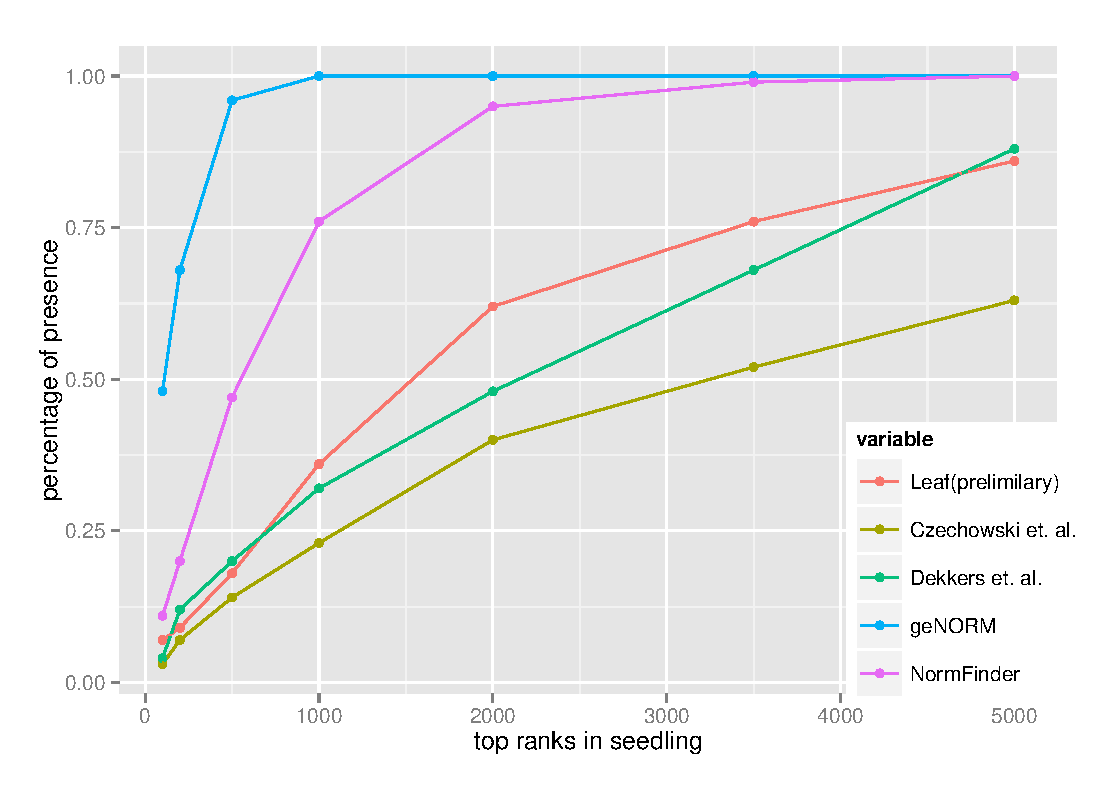
\includegraphics[scale=0.4]{Figures/C1.eps}
%\includegraphics[scale=0.4]{Figures/C2.eps}
%\includegraphics[scale=0.4]{Figures/C3.eps}
%\caption{{\small{\label{sup:expressinlevel} expression levels of Arabidopsis RNA-Seq leaf data: traditional reference genes in set 3 (top)};  5 stably expressed genes by  Czechowski et. al. (middle); 5 stably expressed genes identified by total variance (bottom)}}
%\end{center}
%\end{figure} 


% \begin{figure}[h!]
%\begin{center}
%\includegraphics[scale=0.5]{./Figures/rank_sl.eps}
%\includegraphics[scale=0.5]{./Figures/rank_st.eps}
%\caption{\label{fig:rankAgainstrank} Rank plot of stably expressed genes,  Set 1 versus Set 2 and Set 3.}
%\end{center}
%\end{figure}
%
% \begin{figure}[h!]
%\begin{center}
%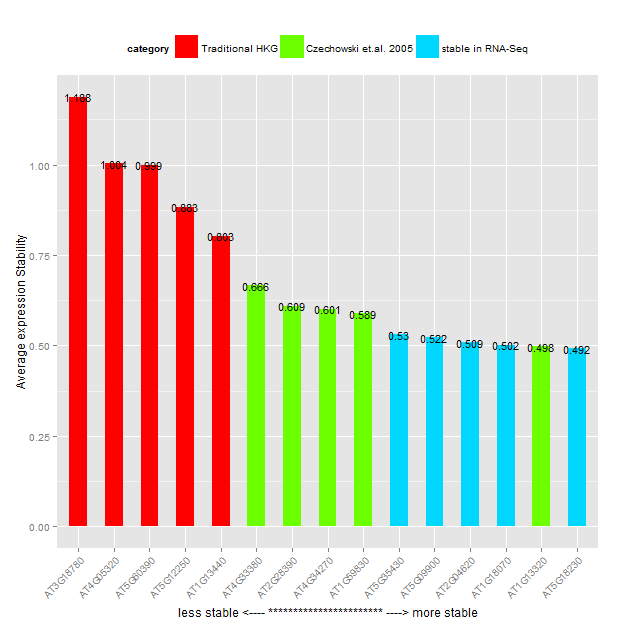
\includegraphics[scale=0.3]{Figures/mvalue2.eps}
%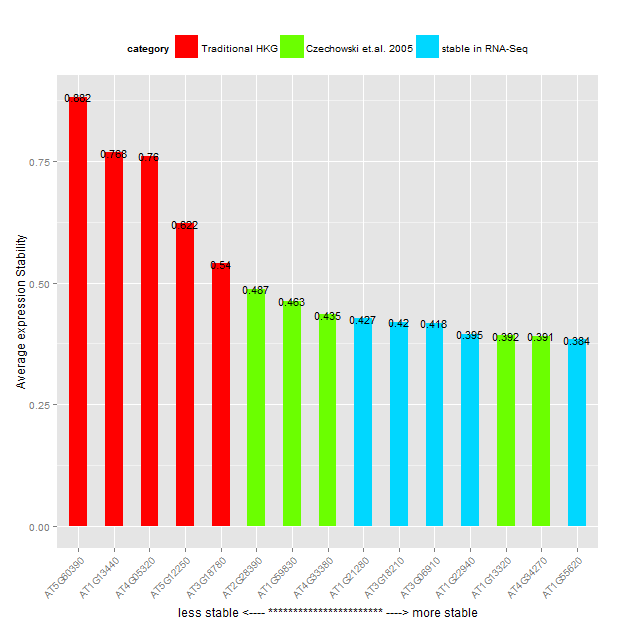
\includegraphics[scale=0.3]{Figures/mvalue3.eps}
%\caption{\label{sup:mvalue} geNORM ranking of reference genes: 5 traditional HKGs, 5 reference genes identified by Czechowski et. al. and 8 stably expressed genes based on seedling RNA-Seq data.  The spearman correlations of $M$-values and total variance  are 0.989 and 0.977, respectively. }
%\end{center}
%\end{figure}


\newpage


%\bibliographystyle{apalike}
\bibliographystyle{DeGruyter-hsk}
%\bibliographystyle{DeGruyter}
\bibliography{mybib}

\end{document}
%
%we randomly choose five genes from top 100 stably expressed genes identified from leaves group, and compared them to five genes randomly chosen from top 100 stably expressed genes of multi-tissue group. Figure \ref{expressinlevel2} displays the expression profiles in CPM over the five experiments in leaves group. Three genes from multi-tissue group show large between-experiment variation in leaves group. As we commented earlier, genes that are stable under a wider range of conditions may not be the most stable ones under a narrow set of conditions.
%
%
%
%\begin{figure}
%\centering
%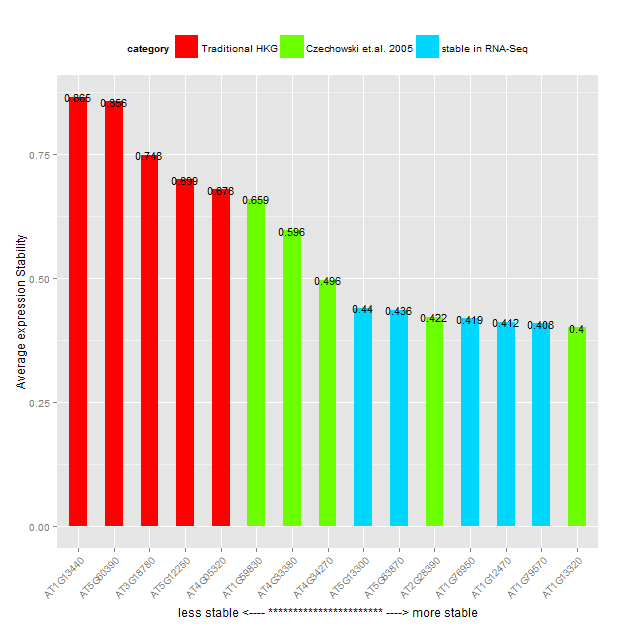
\includegraphics[width=0.7\linewidth]{Figures/mvalue1}
%\caption{}
%\label{fig:mvalue1}
%\end{figure}
%
%
%
% \begin{figure}[H]
% \begin{center}
%	%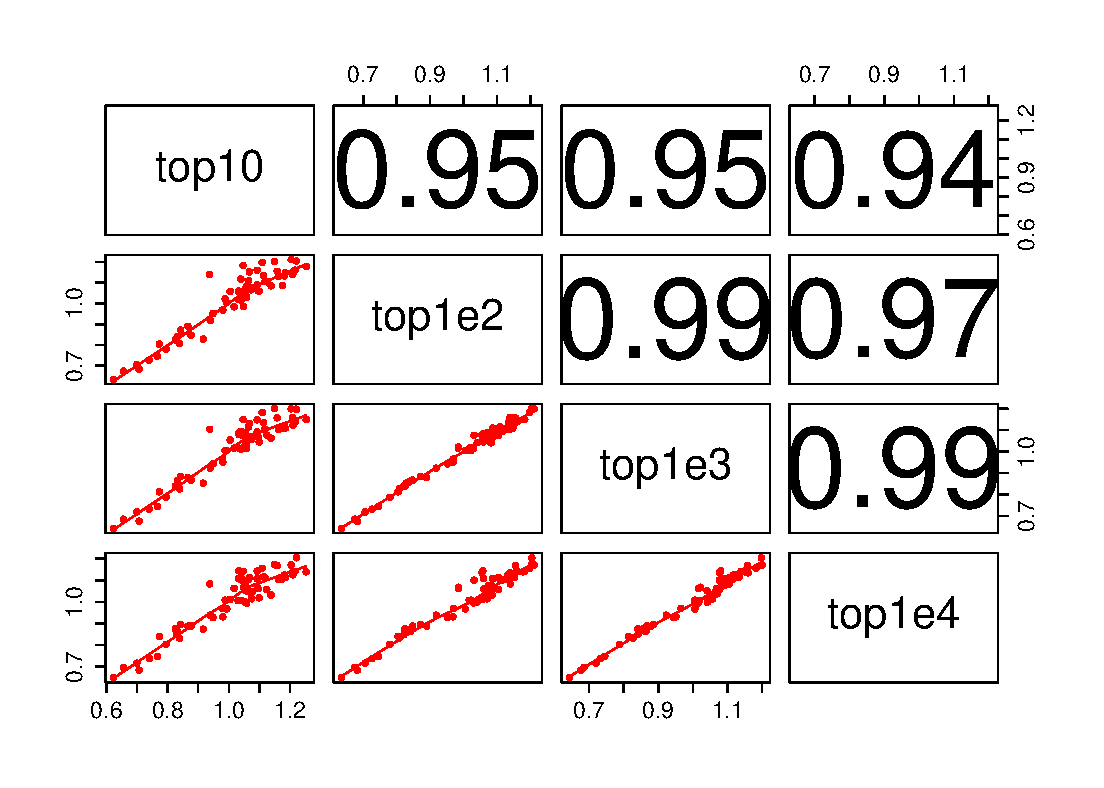
\includegraphics[scale=0.5]{Figures/B1.eps}
%	
%	\includegraphics[scale=0.4][Figures/tissue_leaf.eps}
%	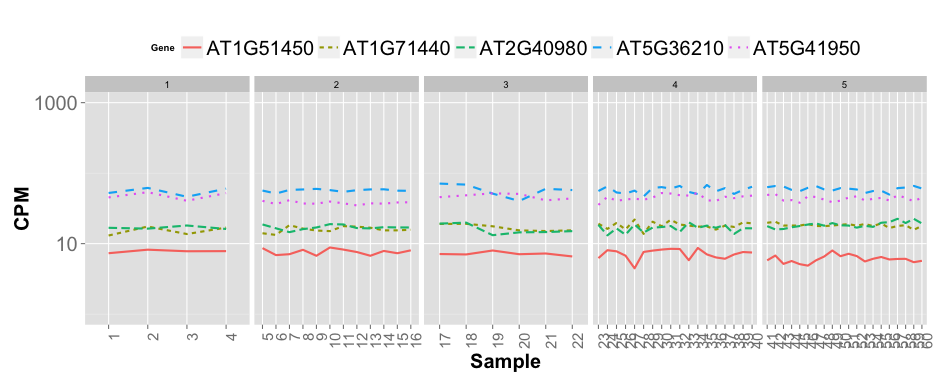
\includegraphics[scale=0.4]{Figures/leaf_leaf.eps}
%	\caption{{\small{\label{expressinlevel2} Expression levels CPM plotted using leaves data: 5 stably expressed genes randomly selected from top 100 of leaves group (top) ; 5 stably expressed genes randomly selected from top 100 of multi-tissue group }}}
%\end{center}
%\end{figure} 
%
%
